\RequirePackage{plautopatch}
\documentclass[dvipdfmx,a4paper]{jsarticle}
\usepackage{amsmath}
\usepackage{amssymb}
\usepackage[dvipdfmx]{graphicx}
\usepackage[margin=20truemm]{geometry}
\usepackage{url}
\usepackage{wrapfig}
% for hyperref
\usepackage[dvipdfmx, bookmarkstype=toc, colorlinks=false, pdfborder={0 0 0}, bookmarks=true, bookmarksnumbered=true]{hyperref}
\usepackage{pxjahyper}
\usepackage{here}

\title{\vspace{-1cm}テクニカルドキュメント}
\author{\texttt{こんぶ畑}}
\date{2024年3月1日}

\begin{document}

  \maketitle
  \section{チーム基本情報}
    
    \subsection{チームコード・チーム名}
    WRS002 こんぶ畑
    \subsection{リーグ}
    Rescue Simulation (Erebus)
    \subsection{国・地域}
    岡山

  \section{チーム情報}
    \subsection{チームについての説明}
    \noindent
    チーム名:こんぶ畑 (こんぶばたけ)

    \noindent
    メンバーの 1 人が所属していた部活の愛称と顧問への敬意を込めて名付けた。\\
    リーダー は高 1、高 2 とレスキューラインに参加してきた。今年度は受験の年で参加は半ば諦めていたが、幸運にも年内に志望校合格を果たし、もう 1 人を連れてくることでチームを結成することができた。\\
    結成は2024年になってからだ。わずか3ヵ月で初めての競技に挑む。

    \subsubsection{情報公開}
    \noindent
    情報公開はロボカップジュニアの国是のようなもだ。\\
    しかし、シミュレーションリーグでコードをオープンにすることは、実機リーグのそれとは持つ意味合いが少し違うと考える。良くも悪くも、たった 1 つの exe ファイルが文字通り「全て」なのだから。だが、RCJJ のコミュニティに何か少しでも貢献できることがあればと思い、今年もソースコードを大会終了後にGitHubで公開することにした。\href{https://github.com/KOMBU-Batake}{リンク}\\
    実際にこのソースコードを公開することで直接誰かの参考になるとはあまり思っていない。それよりも、自分を含めより多くの人が情報公開をすることで、よりコミュニティが活発になることに期待している。

    \subsection{チームの所属団体}
    \noindent
    個人参加

    \subsection{チームメンバー}
    \noindent
    ○○○○(●●●●)\\
    リーダーとしてプログラムの作成をした。\\
    今年こそ最後の大会。悔いのないように頑張りたい。\\

    \vskip.5\baselineskip
    \noindent
    □□□□(■■■■)\\
    突然誘われた一般人\\
    プログラム関連は無知\\
    フィールド作成、ポスターのデザイン提案、修正を行った。
  
  \section{ロボットの構成}
    \subsection{ロボットの写真}
    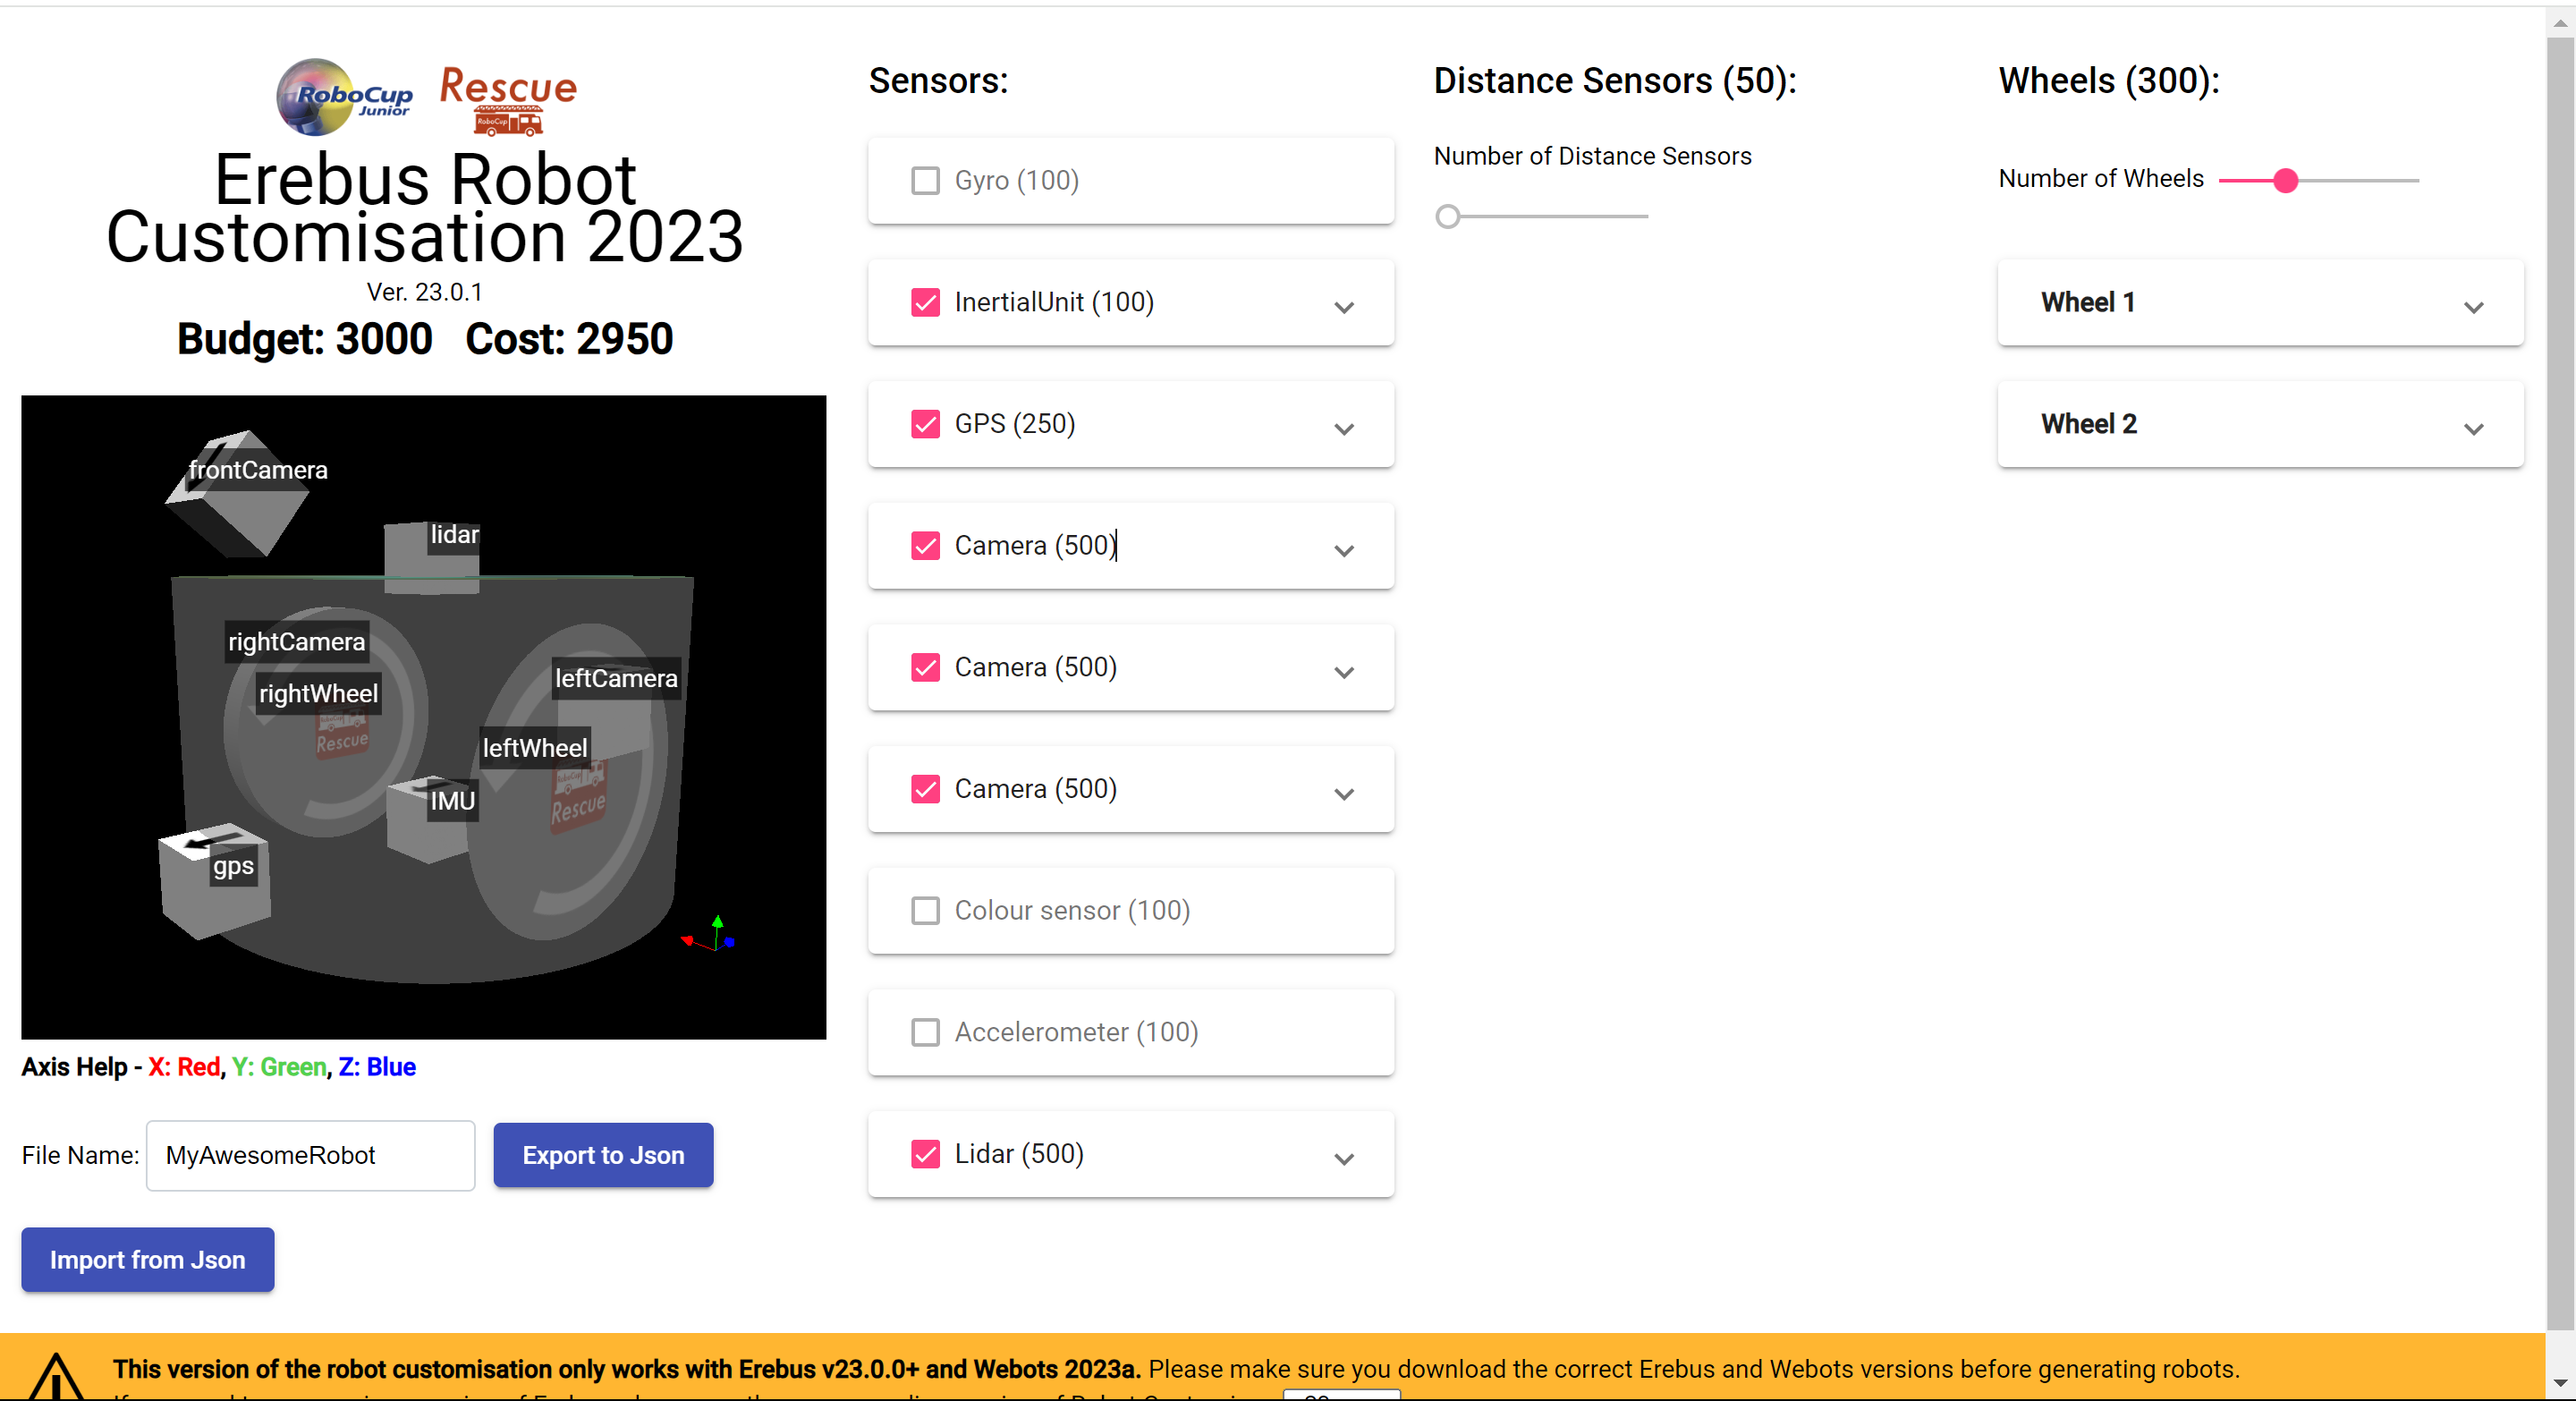
\includegraphics[width=150mm]{Photo/robot.png}

    \subsection{ロボット全般の説明}
    タイヤ・モータの数はそれぞれ2つ。Robot Customizationの標準設定をそのまま使っている。

    \subsection{使用しているセンサーと使用目的}
    \begin{itemize}
      \item 左右モータ + エンコーダ\\
      標準のものをそのまま使用している。\\
      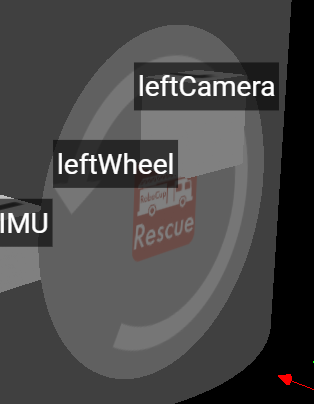
\includegraphics[width=40mm]{Photo/Parts/ダウンロード.png}
      \item IMU\\
      角度を取得するために使用している。\\
      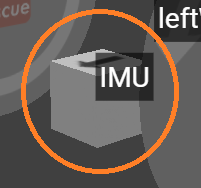
\includegraphics[width=40mm]{Photo/Parts/ダウンロード1.png}
      \item GPS\\
      位置情報を取得するために使用している。\\
      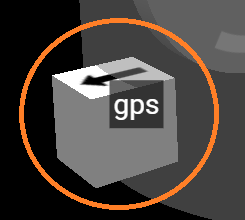
\includegraphics[width=40mm]{Photo/Parts/ダウンロード2.png}
      \item LiDAR\\
      障害物の検知、壁の認識に使用している。\\
      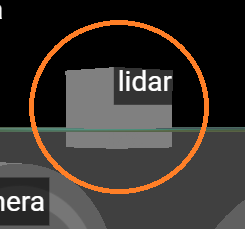
\includegraphics[width=40mm]{Photo/Parts/ダウンロード3.png}
      \item 左右カメラ\\
      被災者の検知に使用している。\\
      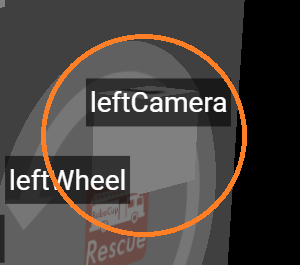
\includegraphics[width=40mm]{Photo/Parts/ダウンロード4.png}
      \item 正面カメラ\\
      障害物を発見と床の色の認識に使用している。\\
      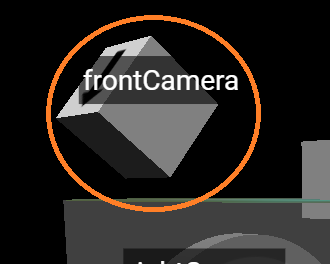
\includegraphics[width=40mm]{Photo/Parts/ダウンロード5.png}
    \end{itemize}
  
    \subsection{被災者の探索}
    \noindent
    正面と左右に1つずつカメラを搭載している。
    \vskip.5\baselineskip
    \noindent
    正面カメラ\\
    斜め上から目の前のタイル1枚を俯瞰するように設置してる。\\
    Fov(視野角)を標準の1radから1.5radに広げて使用している。
    \vskip.5\baselineskip
    \noindent
    側面カメラ\\
    被災者に対して水平な高さから、被災者がちょうど収まるくらいの位置に置いている。
  
  \section{ロボットのソフトウェア}

    \subsection{使用しているプログラミング言語・ソフトウェア}
    \noindent
    主な開発環境
    \begin{itemize}
      \item Webots 2023.a
      \item Erebus v23.0.5
      \item C++ 14 (メイン言語)
      \item Python 3.12.1
      \item Visual Studio 2022
    \end{itemize}

    使用した言語はC++である。殊レスキューシミュレーションにおいてはPythonの方がポピュラーであることは何となしに知っていたが、C++の方が好みなのでC++を採用した。\\
    もちろん、画像認識の選択肢が狭まることは承知の上である。\\

    Visual Studioの環境構築には苦労した。なにせ、レスキューシミュレーション公式サイトにもDiscordにも情報がないのである。結果的には、Webotsの公式サイトの情報を基に作成した。このままではよくないと思い、簡単にだが環境構築方法をまとめたページを作成した。\href{https://qiita.com/kikou0517/items/f13045b6b97767e7d0f0}{リンク}\\
    
    ソースコードの管理にはGitHubを使用した。draw.ioで作成したポスターと合わせて管理している。\\
    ブランチ戦略にはGitHub Flowを使用している。かつてはgit-flowを使用していたが、今回は小規模開発のためシンプルで細やかなリリースを重ねていける開発スタイルを選択した。\\
    他にも、GitHubのProject機能を使ったタスク管理を行うこともできた。\\
    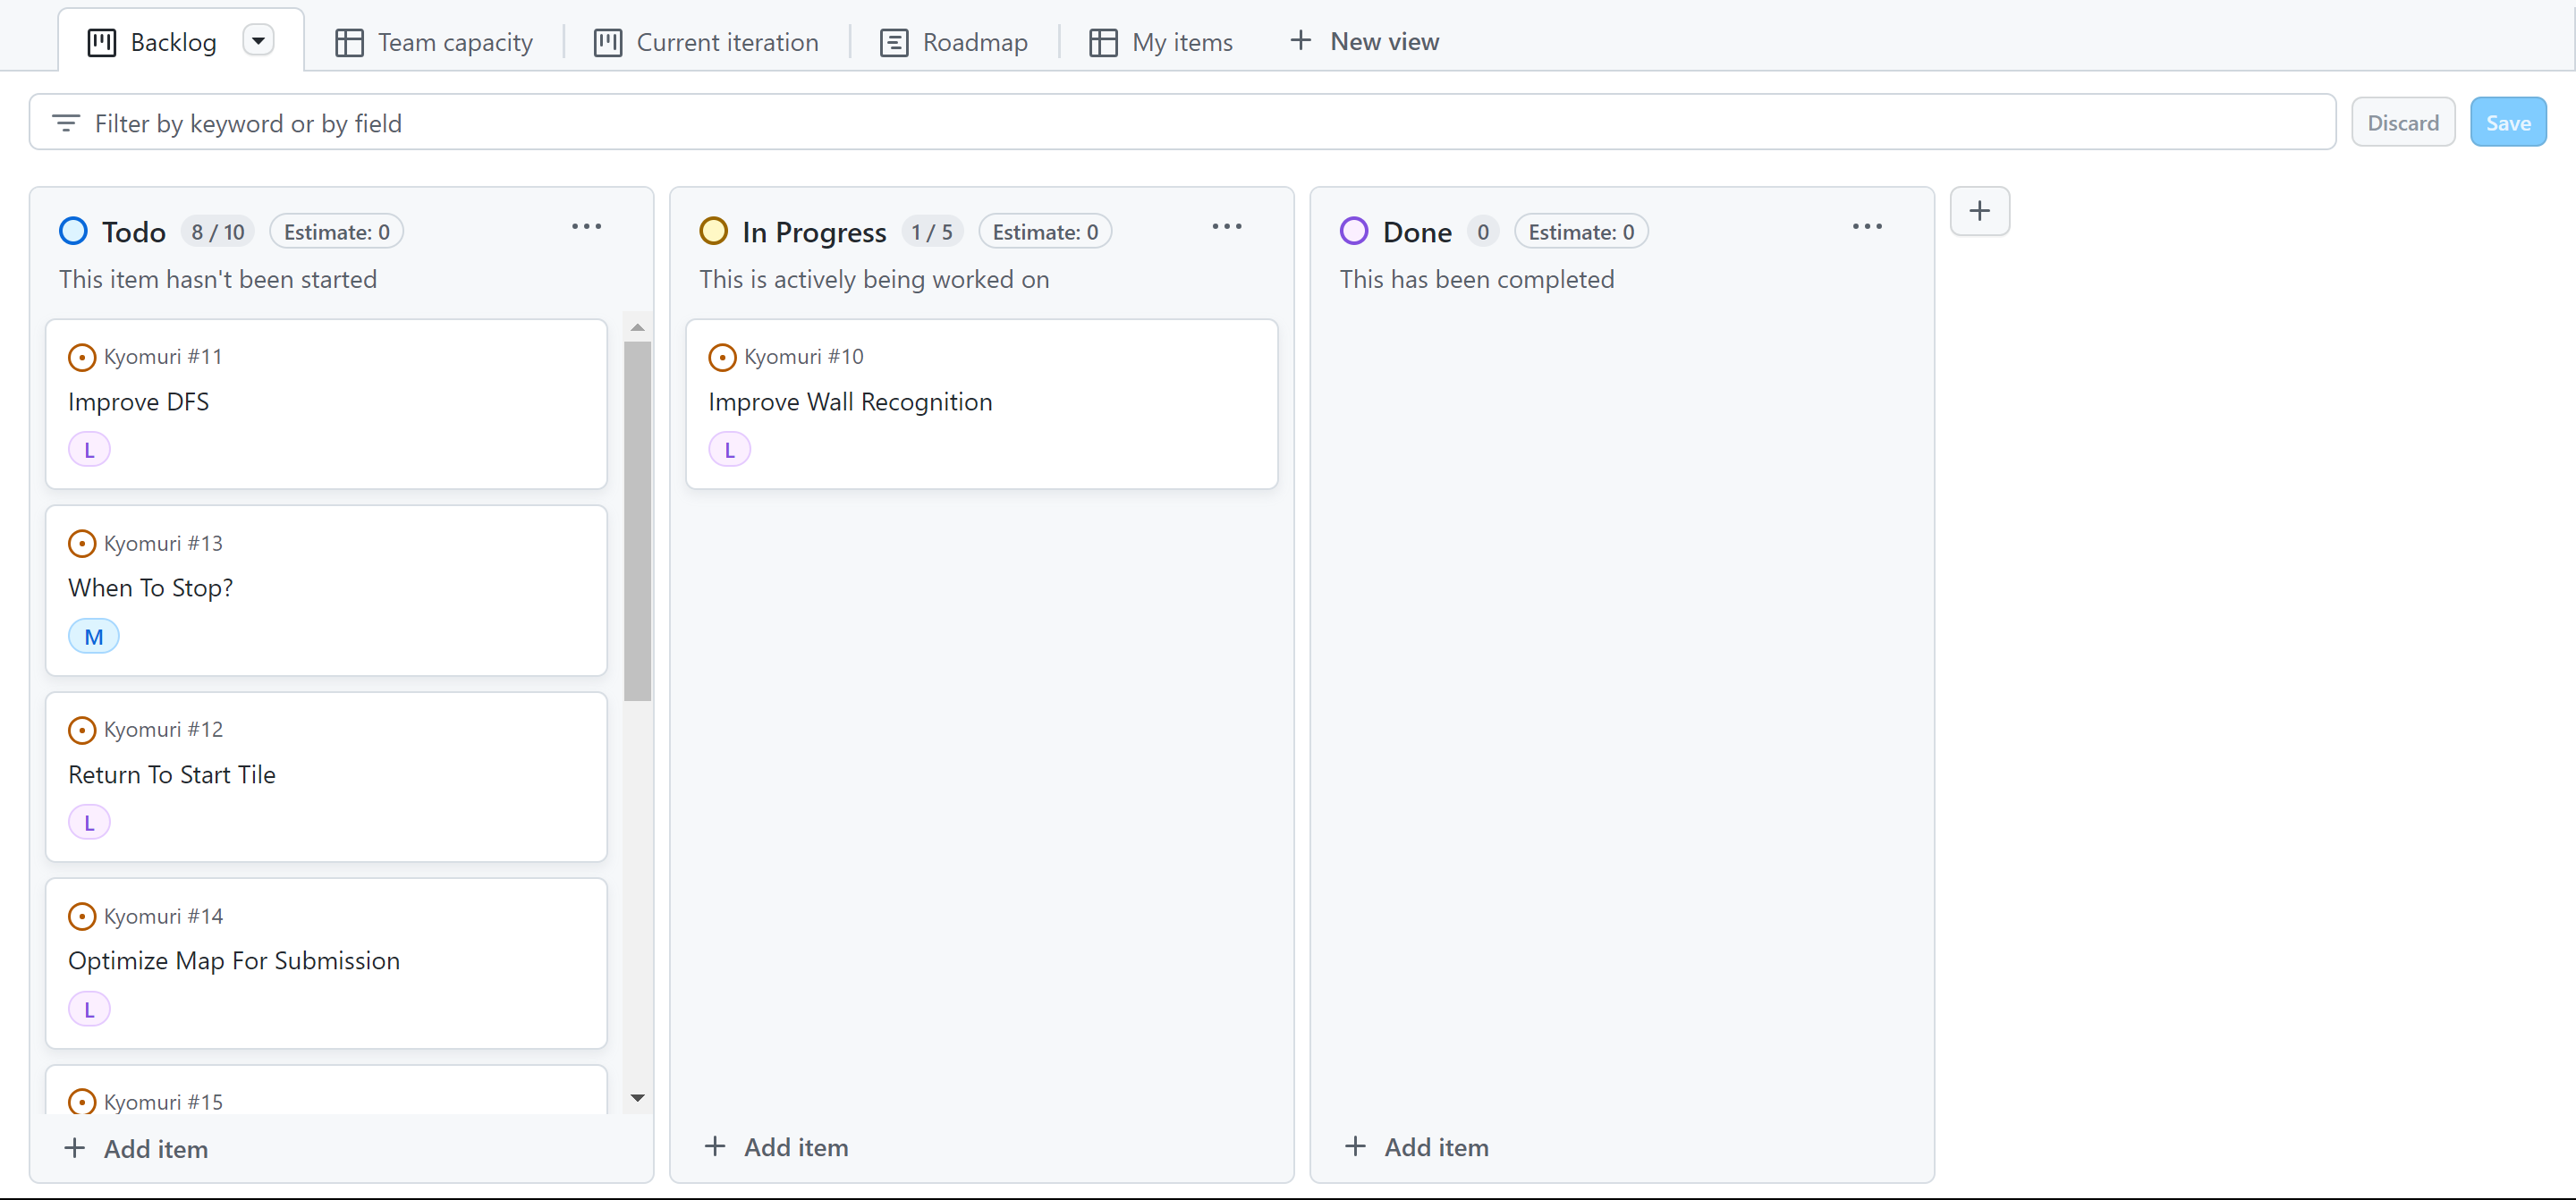
\includegraphics[width=150mm]{Photo/1.png}

  \subsection{迷路探索}

    \subsection{探索アルゴリズム}
    深さ優先探索を使用する。探索は6cm単位で行う。\\
    オリジナルの工夫点も加えた。\\
    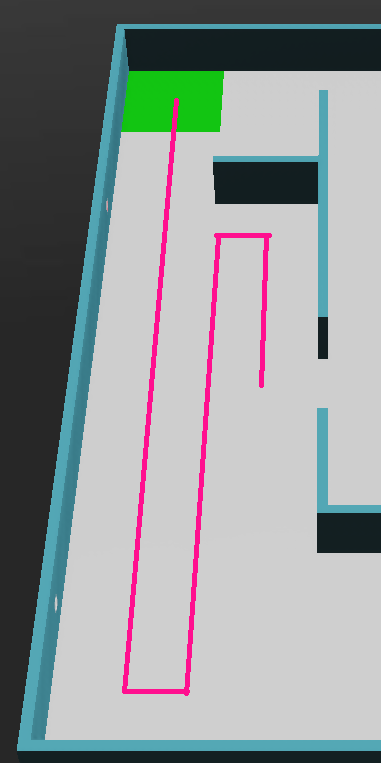
\includegraphics[width=40mm]{Photo/feagure1.png}
    \noindent
    上図のマップでは、ピンク線で示したように探索済みのマスを半分跨ぎながら進むという効率の悪い探索を行う可能性がある。これは機体のサイズは12$\times$12cmを基準とするのに対して、6cm単位で探索を行うことが原因である。\\
    そこで深さ優先探索における「未探索」「探索済み」という2つのパラメーターに「部分的に探索済み」を加え、進行方向の候補が複数あった場合に「部分的に探索済み」の優先度を下げることで、上図のような探索を防いでいる。\\

    \subsection{マッピング}
    \noindent
    vector配列で随時拡張しながら、提出するマップと同じ形式で記録する。\\
    このマップは深さ優先探索や幅優先探索で最短経路を求めることにも使う。

    \subsection{LiDARの活用}
    LiDARってなんか難しそう。でも使えればこれ以上の味方はいない。
    \subsubsection{値の補正}
    \noindent
    搭載されているLiDARから取得できるデータは全体を4周できる分だけあり、それぞれ512個ずつ存在する。それぞれY軸方向に対する向き(もしくは位置)の違いがあり、4周のうち3周目が最も適切に距離関係を示していたためこれを使用している。\\
    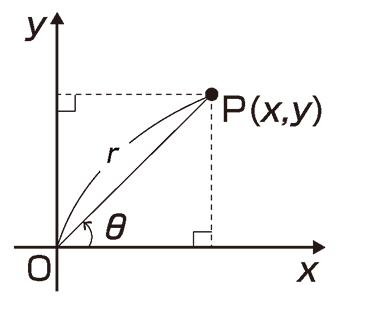
\includegraphics[width=30mm]{Photo/LiDAR/2.png}\\
    LiDARのデータは極座標だと考えることができる。
    それをXZの直交座標に変換して扱う。\\
    また、以降において軸の表記がないグラフは縦軸を上側正のZ軸、横軸を右側正のX軸とする。\\
    また、ロボットが毎回理想的な位置でデータを取得できるとは限らない。少なからず「角度」「位置」のずれが生じるはずだ。\\
    ロボットから見た点群とフィールドの地形を同列に扱うには点群の補正が不可欠である。\\

    \noindent
    まず、回転方向のズレを修正する。左の図が修正前、右の図が修正後だ。\\
    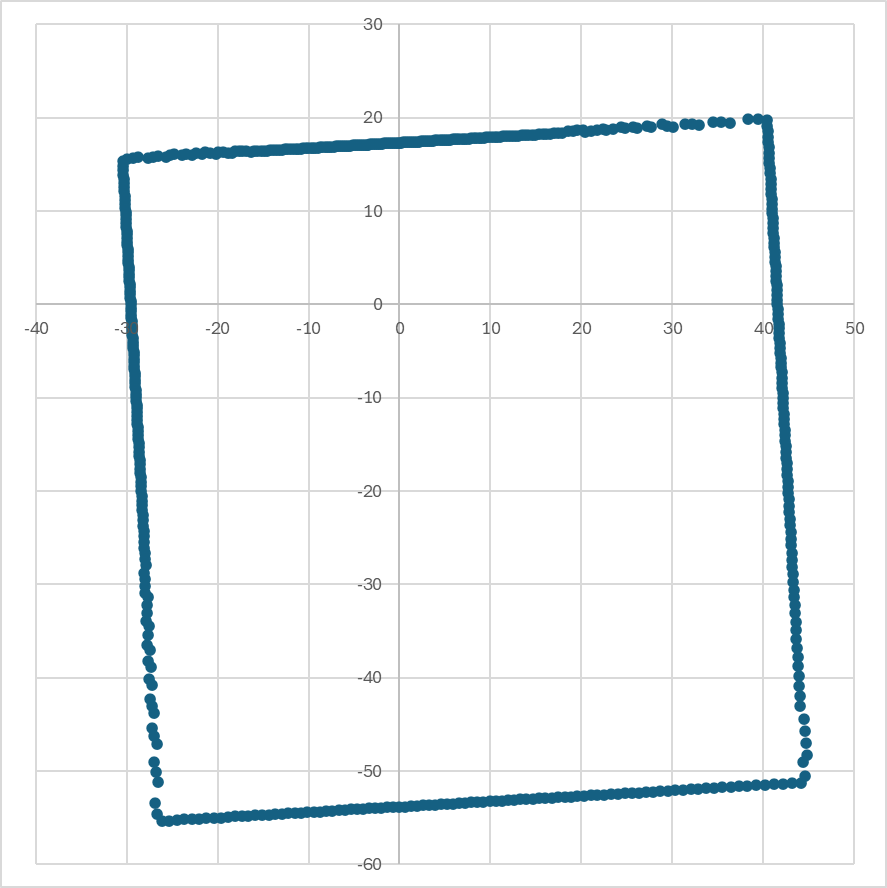
\includegraphics[width=50mm]{Photo/LiDAR/3-1.png}
    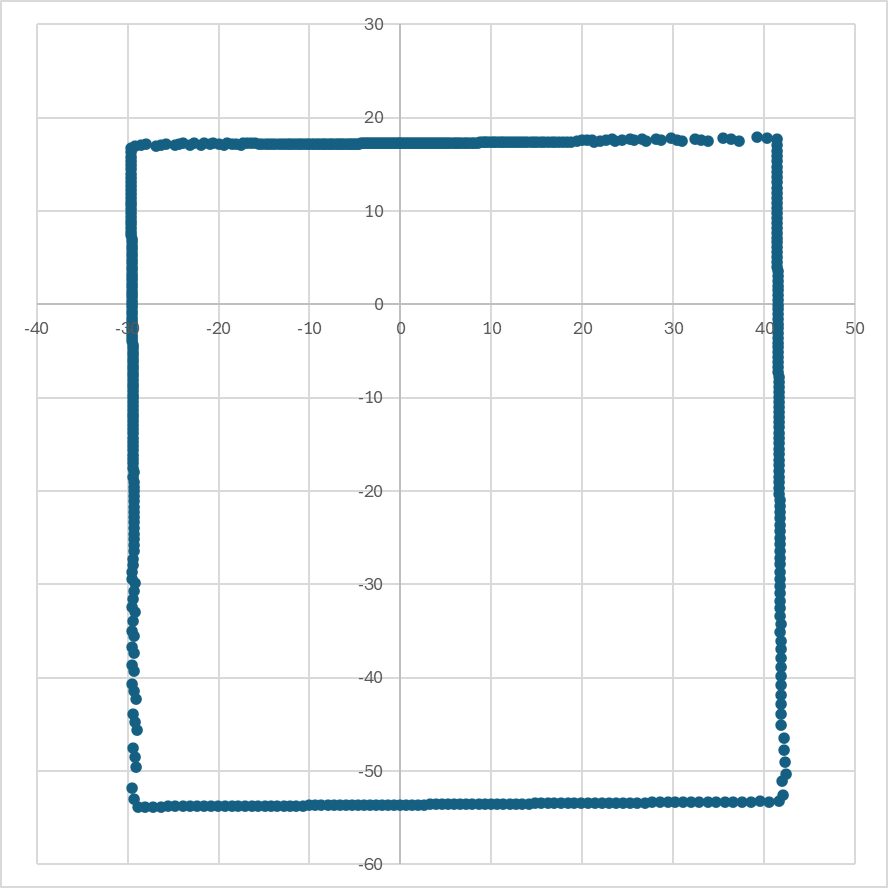
\includegraphics[width=50mm]{Photo/LiDAR/3-2.png}\\
    この修正には回転行列を用いて計算する。
    $$
    \begin{pmatrix}
    X\\
    Y
    \end{pmatrix}
    =
    \begin{pmatrix}
    \cos\theta & -\sin\theta \\
    \sin\theta & \cos\theta
    \end{pmatrix}
    \begin{pmatrix}
    x\\
    y
    \end{pmatrix}
    =
    \begin{pmatrix}
    x\cos\theta - y\sin\theta \\
    x\sin\theta + y\cos\theta
    \end{pmatrix}
    $$

    \noindent
    次に位置の補正をする。\\
    理想的な位置とGPSから得られた実際の位置の差を計算し、LiDARの点群の原点を理想的な位置に合わせる。

    \subsubsection{壁の認識}
    \noindent
    前後左右の隣のマスの壁の種類を判別する。
    
    \begin{enumerate}
      \item 調べる方向12cmのデータを点群から切り取る\\
        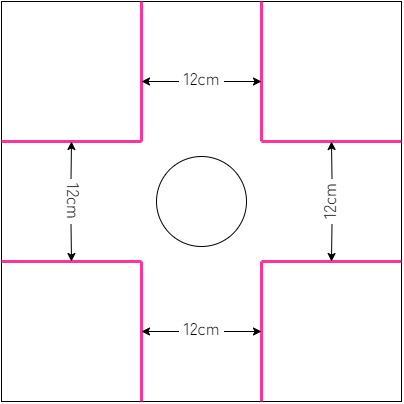
\includegraphics[width=50mm]{Photo/LiDAR/4.png}
      \item 点群を回転させる\\
        このままでは切り取った点群は東西南北各々の方向を向いているので、それを機体から見て前の方向に回転させる。\\
        こうすることでこの後の処理において条件分岐を少なくすることができる。
      \item ベクトルトレーサー法を用いて特徴点を抽出する。\\
        使用しているベクトルトレーサー法は\href{https://www.jstage.jst.go.jp/article/jsprs/48/5/48_5_308/_pdf}{この文献}を参考に作成した。\\
        \begin{quote}
          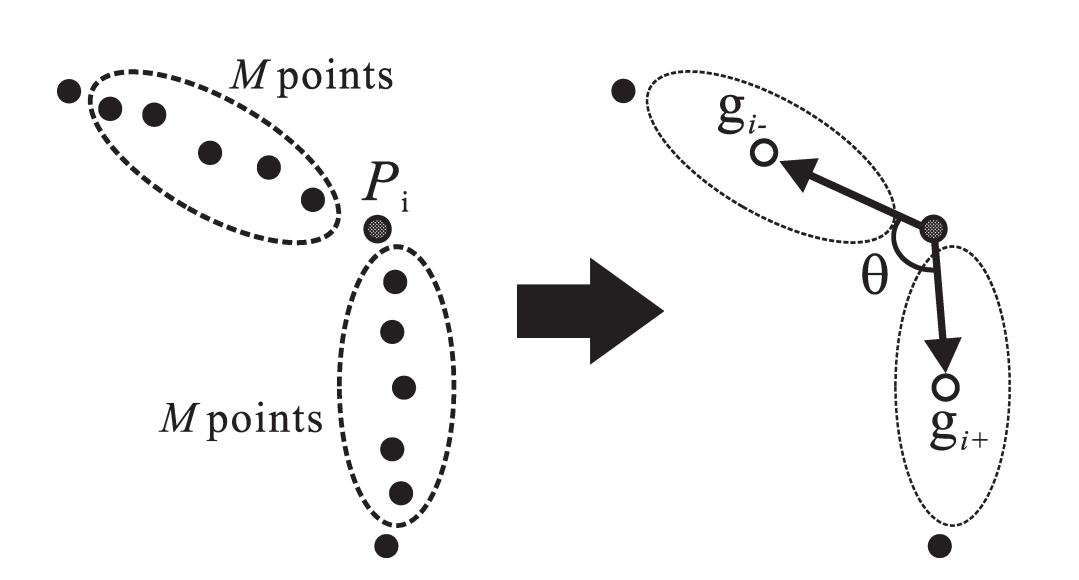
\includegraphics[width=70mm]{Photo/LiDAR/5.png}
        \end{quote}
        ある点Piの前後2点の重心gi+,gi-を求め、これら3点のなす角θを内積を使って求める。\\
        このままでは1つの特徴点に対して複数が抽出される場合がある。そこで連続して抽出された特徴点はθが最大のものを代表値として扱う。\\
        しかし、下の場合の様に特徴点が連続して抽出されることが正しい場合もある。\\
        
\includegraphics[width=30mm]{Photo/LiDAR/6.png}
        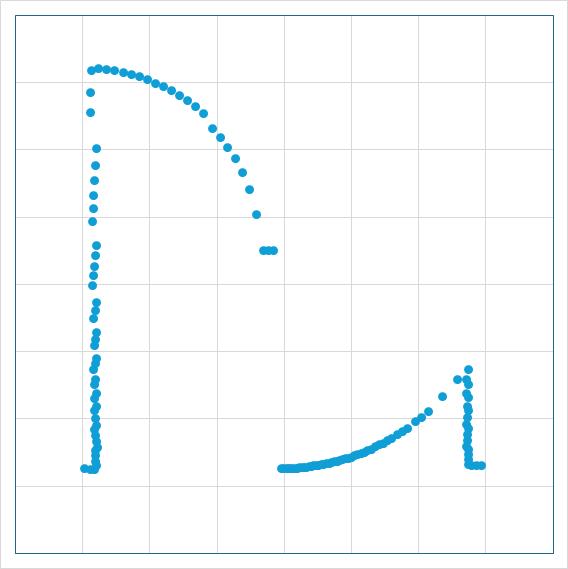
\includegraphics[width=30mm]{Photo/LiDAR/7.png}\\
        そこで$P_i$を原点とした$g_{i+}$ベクトルと$g_{i-}$ベクトルの和であるsベクトルがX軸となす角$a$を定義する。$a_n$の値が$a_{n-1}$と大きく違う場合は別の特徴点とみなす。\\
        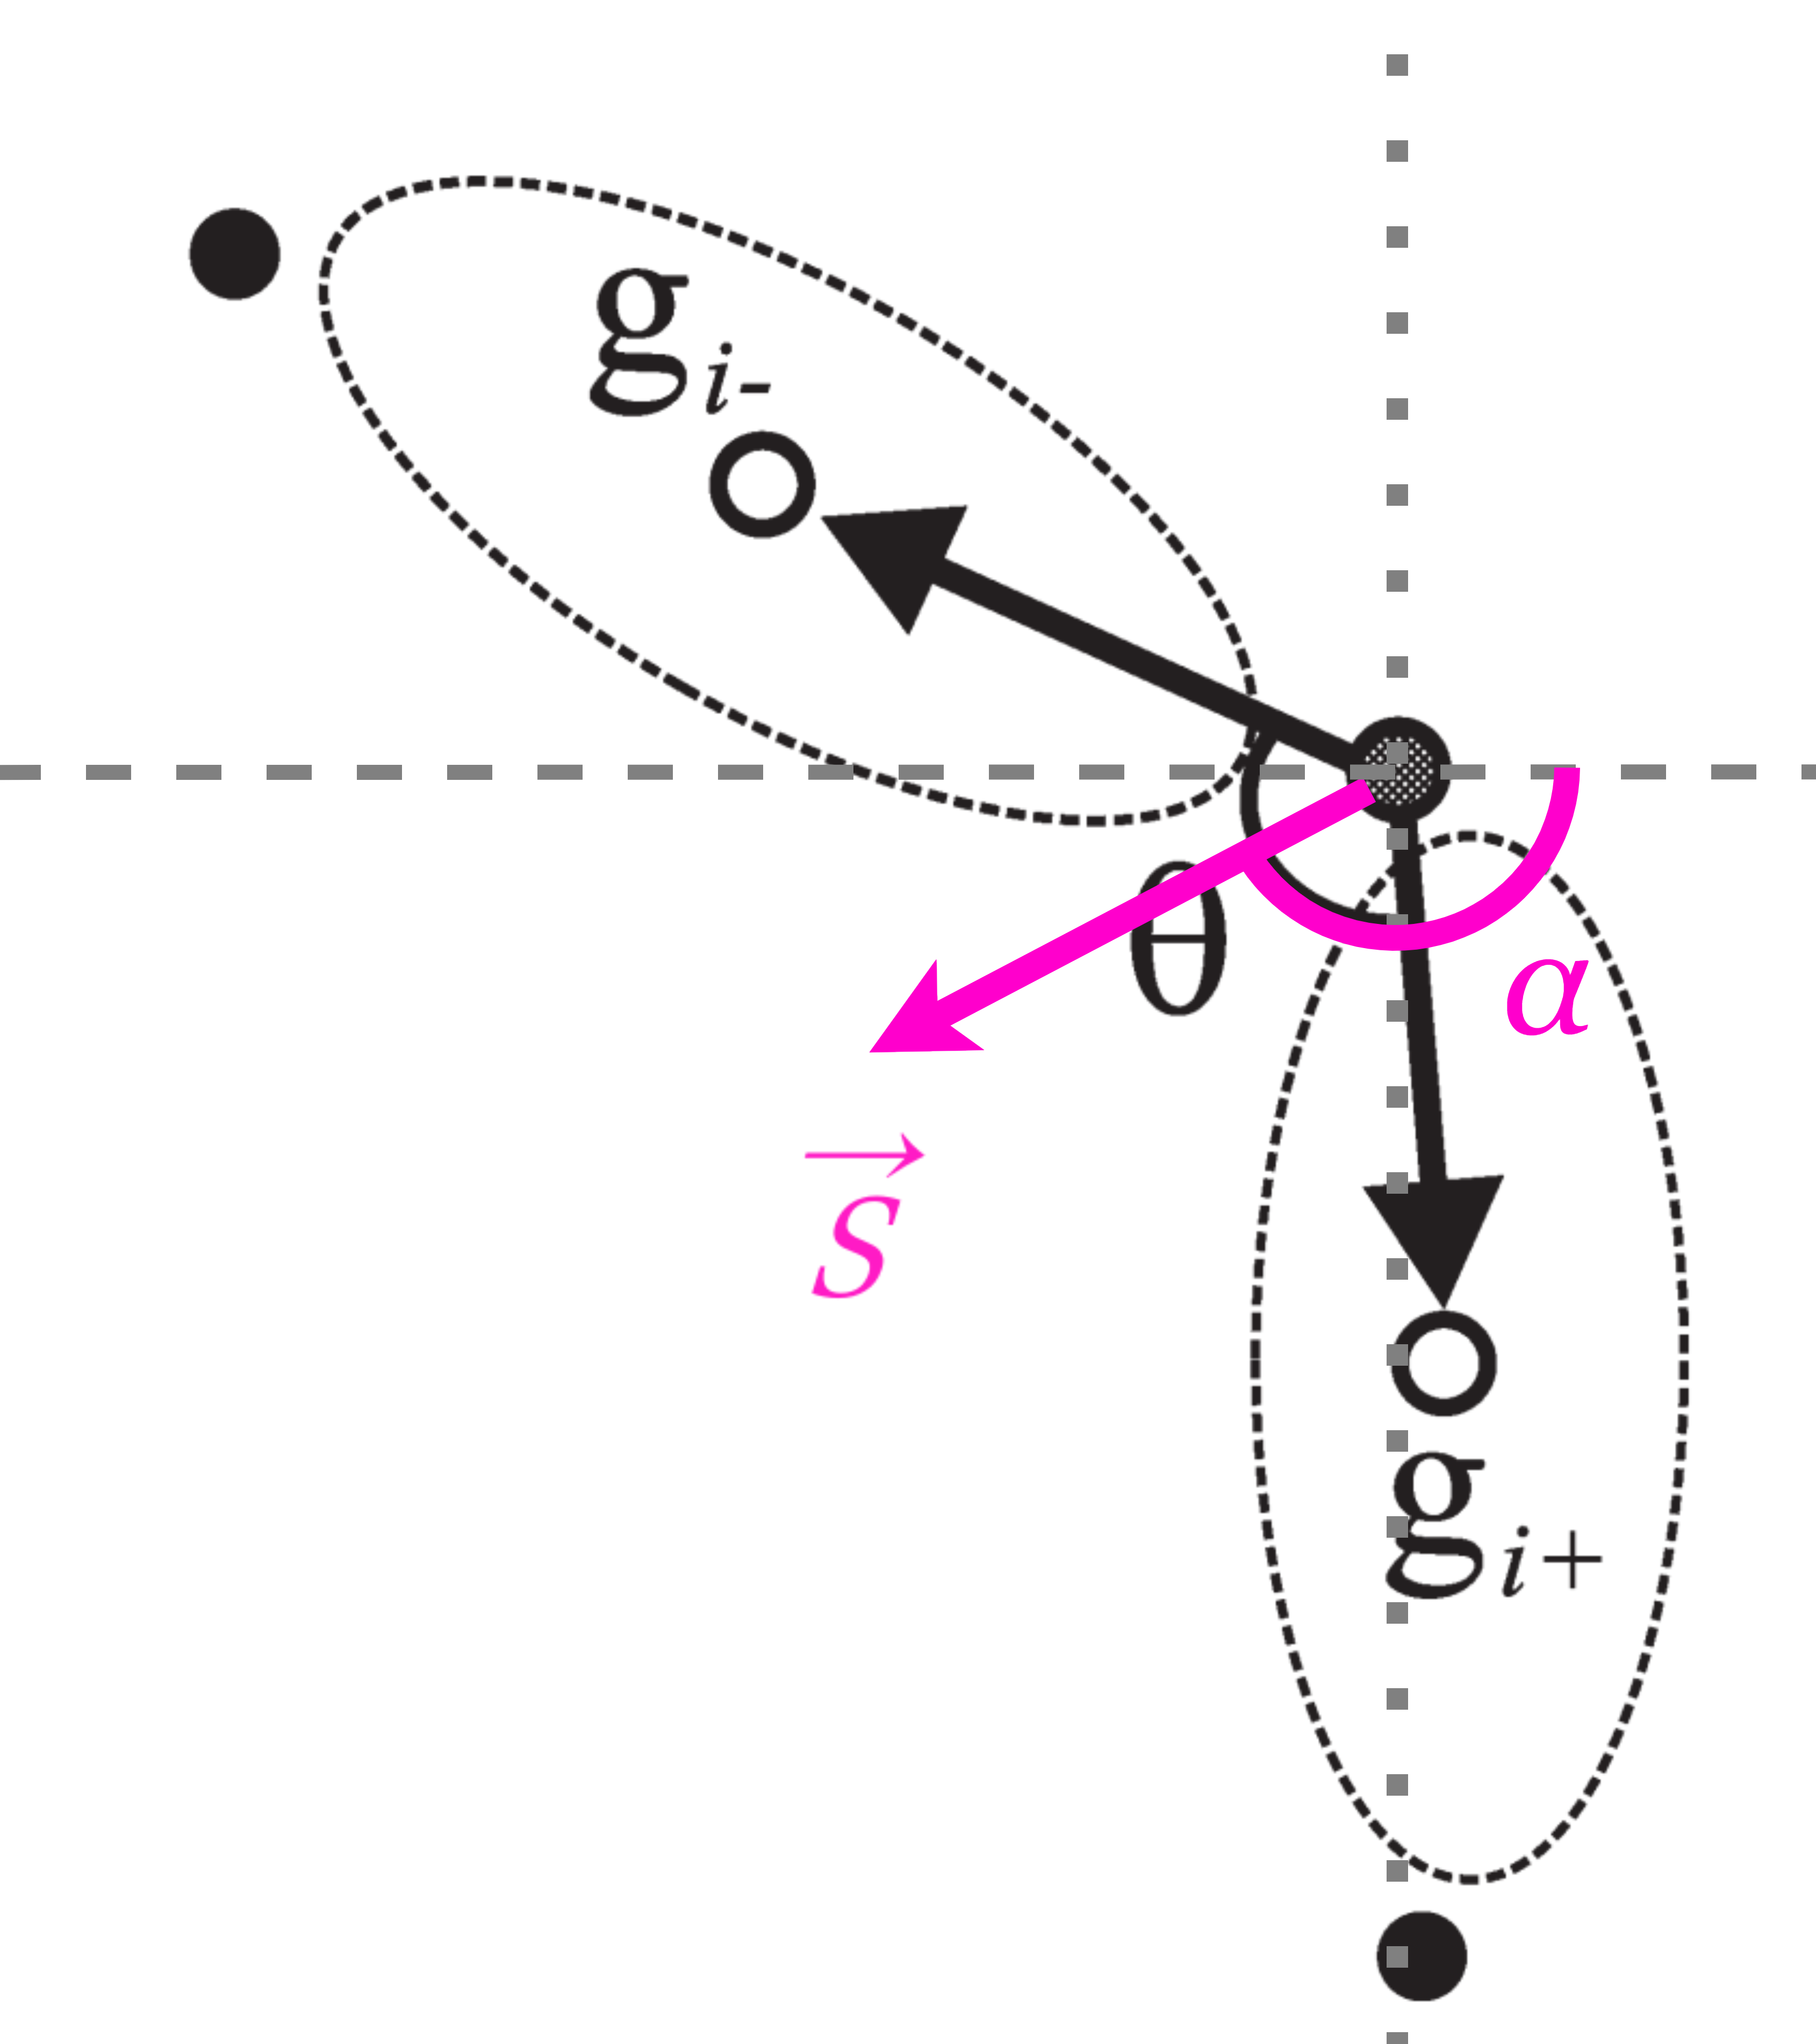
\includegraphics[width=40mm]{Photo/LiDAR/8.png}\\
        これまでのプロセスを経て抽出された特徴点が下の画像中のオレンジ色の点である。\\
        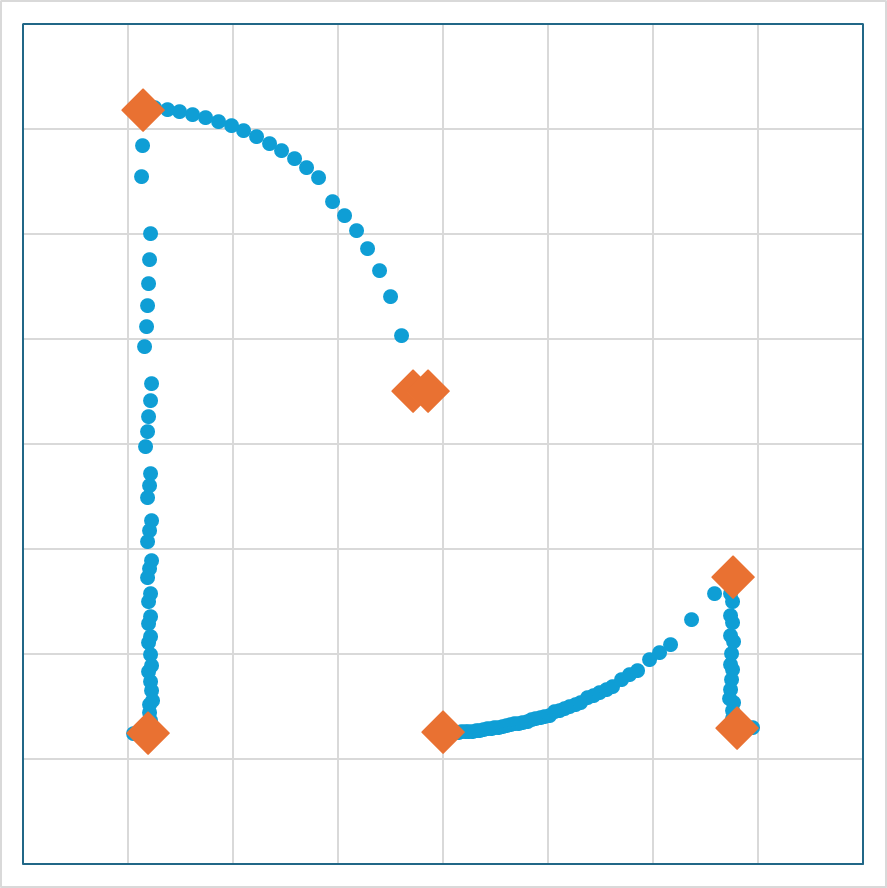
\includegraphics[width=40mm]{Photo/LiDAR/9.png}
      \item 判定する範囲の決定\\
        この点群において壁の種類を判定するのに必要なのは円で囲った範囲である。これの左右の範囲の判定には先ほどの特徴点を使う。\\
        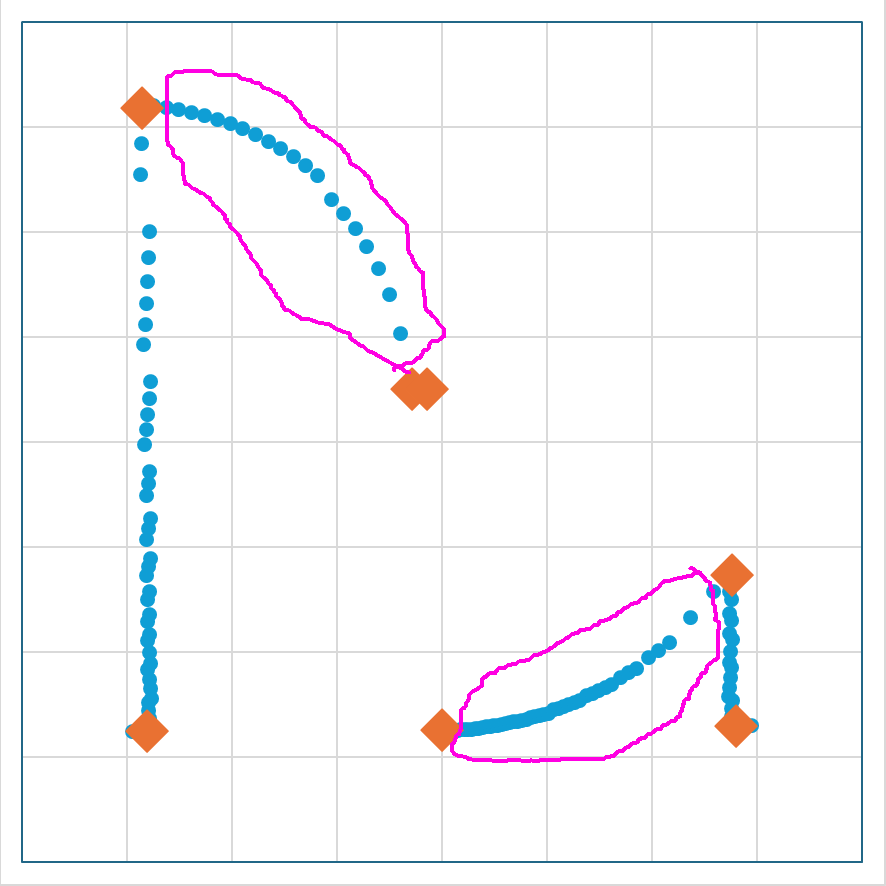
\includegraphics[width=40mm]{Photo/LiDAR/10.png}\\
        左側について、下の図の四角形で囲んだ領域内に特徴点があった場合、その中で最も端から離れたものを始点・終点として範囲を決定する。右側についても同様のことを行う。\\
        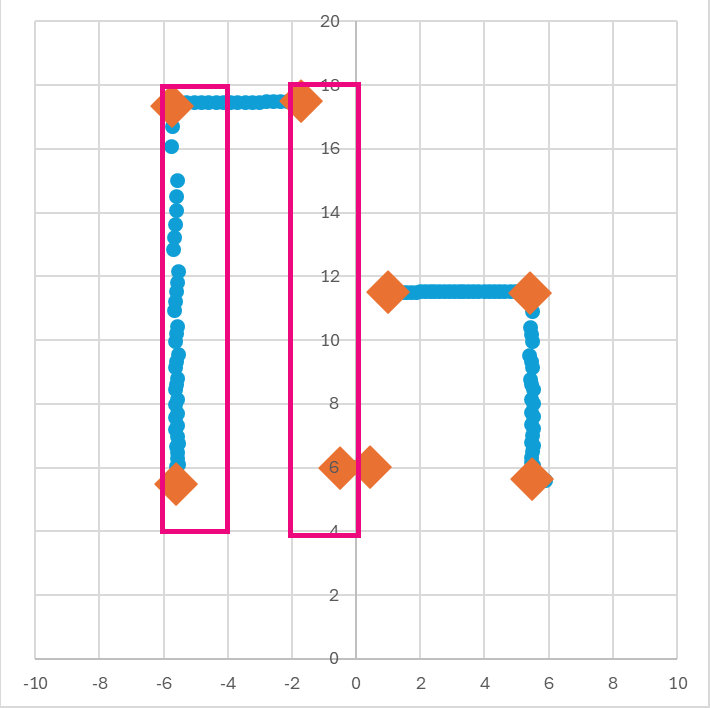
\includegraphics[width=40mm]{Photo/LiDAR/11.png}
      \item 判定対象の有無\\
        先ほど決定した範囲の最大値を求め、これが18cmよりも大きい場合は判定対象外とする。
      \item まっすぐな壁であるか\\
        図10のようなまっすぐな壁であるかどうかを判定する。\\
        そのために4. で決定した範囲内の点のZ座標の分散を計算する。まっすぐな壁であればZ軸の値はほぼ一様であり、分散は小さくなる。
      \item 曲線の決定\\
        6. において直線の壁でないと判定された場合は、壁は曲線であると考えられる。その曲線がどこを中心とするかによって4パターンに分けられる。\\
        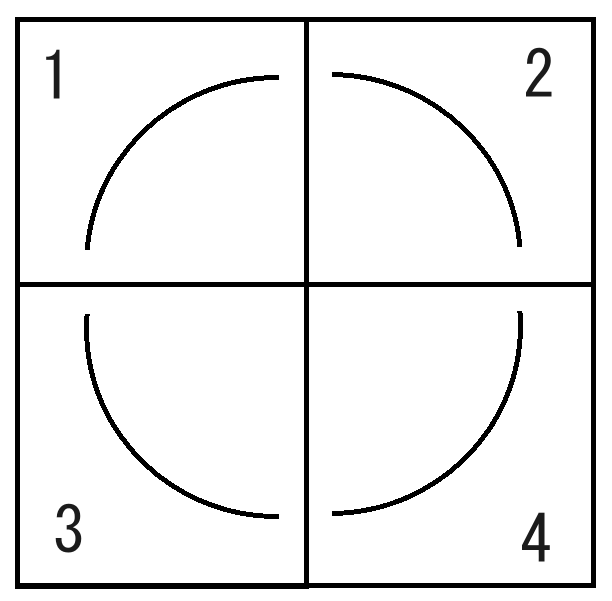
\includegraphics[width=40mm]{Photo/LiDAR/12.png}\\
        まず、右端と左端のZ座標を比較すれば、"1,4"と"2,3"を分けることができる。\\
        ここからさらに分類するために微分する。\\
        例えば、"1 or 4"と判定された対象の場合、壁の測定結果を微分すると"1"ならば減少関数、"4"ならば増加関数となる。これを右端と左端の傾きを比較することで実現する。\\
        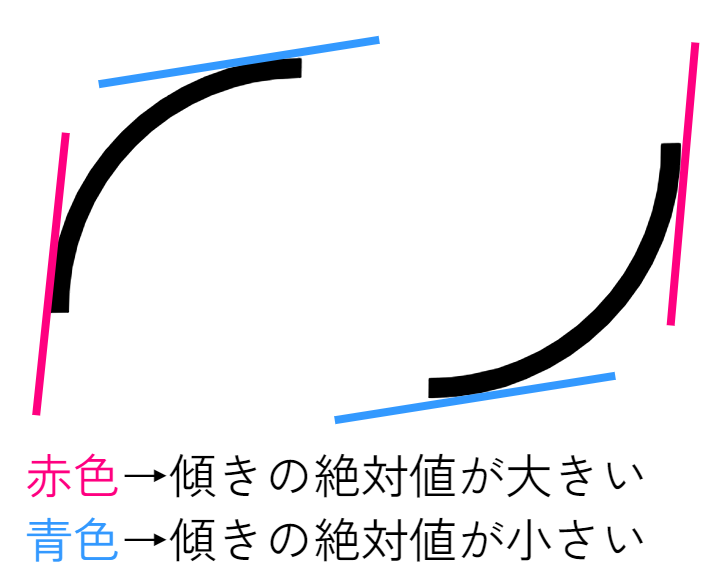
\includegraphics[width=50mm]{Photo/LiDAR/13.png}
      \item 中央の壁\\
        これまでの認識で、中央の壁に覆いかぶさるものがないと判断した場合にのみ中央の壁の認識をする。
        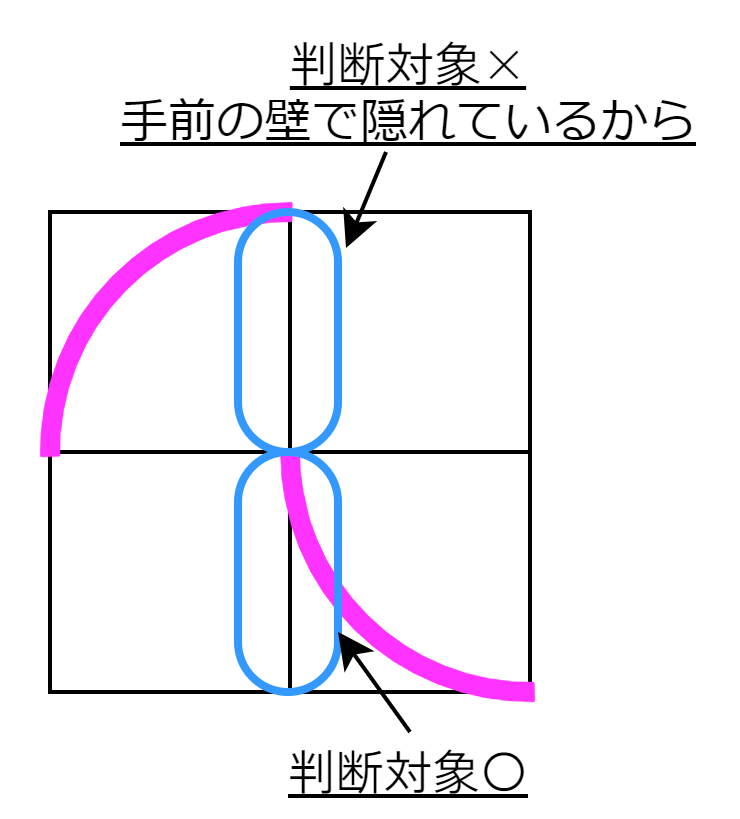
\includegraphics[width=40mm]{Photo/LiDAR/14.png}\\
        最もX座標が0に近い点のZ座標を元にその有無を判断する。
      \item 斜めに進むという選択肢\\
        探索アルゴリズム内では下の写真の様にどうしても斜め前に進まなければいけない場合がある。\\
        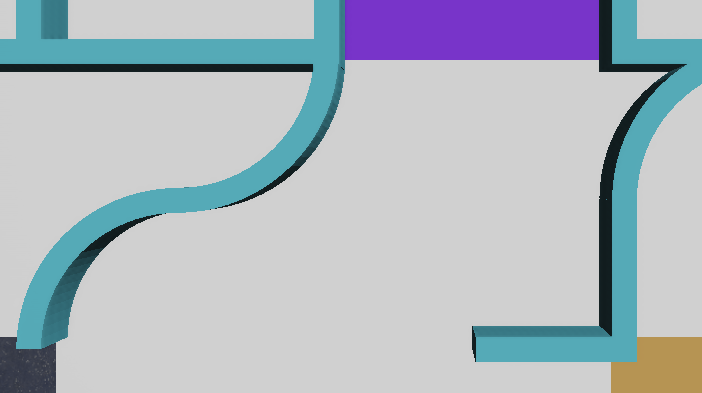
\includegraphics[width=60mm]{Photo/LiDAR/15.png}\\
        斜めに進めるかどうかを判断するために、直径7cmの円を仮想的に斜め前のタイルの中心に置く。そして円の中に点がなければ、進むことができると判断する。\\
        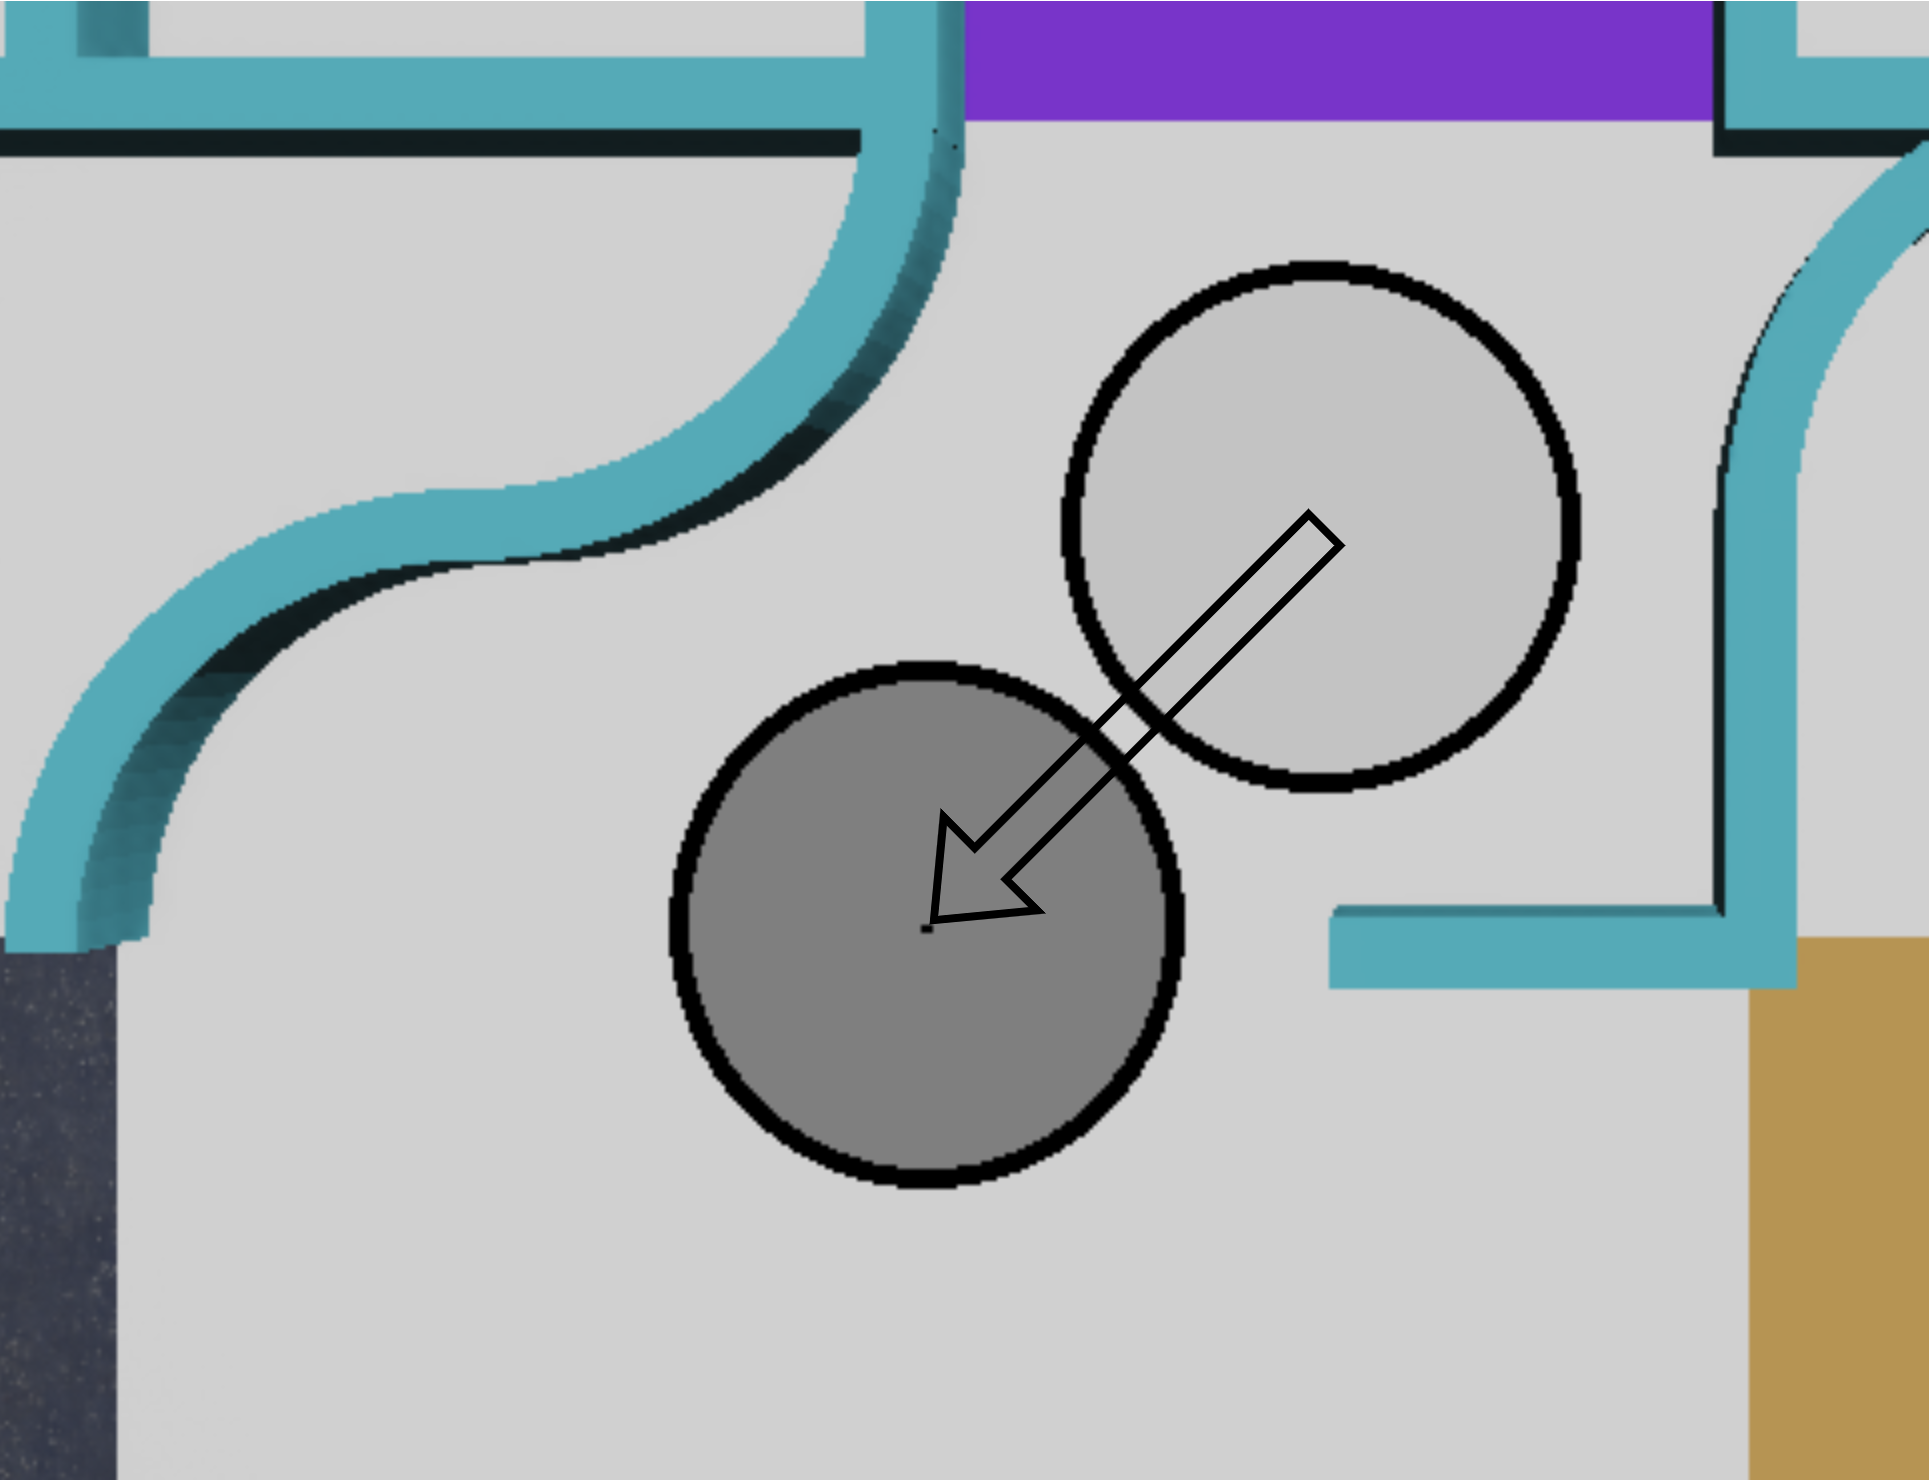
\includegraphics[width=60mm]{Photo/LiDAR/16.png}
    \end{enumerate}

    \subsubsection{障害物の検知 with カメラ}
    LiDARだけで障害物を探すのは無謀だ。サイズ、位置、あまりにもパターンが多すぎる。\\
    しかし、カメラに視点を移せば障害物は明確な特徴を持っている。壁は青に寄った色をしているが、障害物は彩度0だ。これを利用して障害物を探す。
    \vskip.5\baselineskip
    このマップを例に取ってみよう。\\
    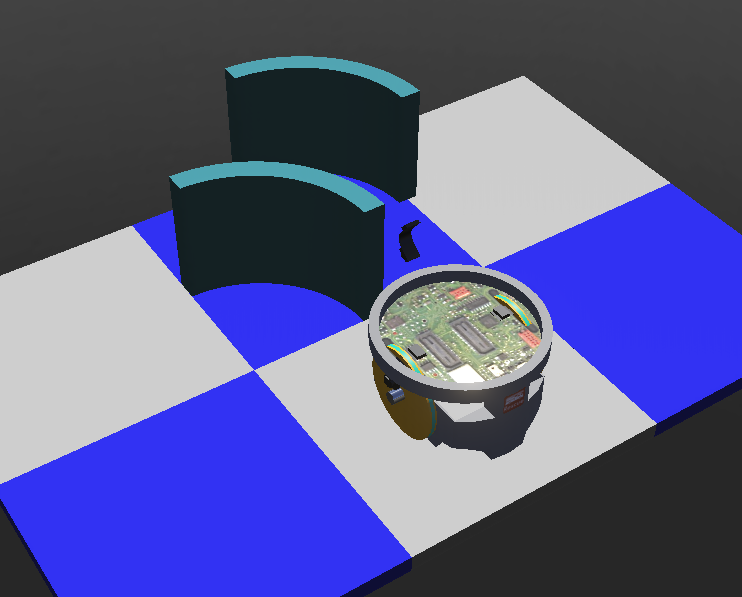
\includegraphics[width=50mm]{Photo/LiDAR/17.png}\\
    正面カメラを使って撮影されたのが下の写真だ。\\
    
\includegraphics[width=50mm]{Photo/LiDAR/18.png}\\
    しかしこれは鳥瞰画像ではないため扱いづらい。\\
    そこで射影変換を用いて修正する。\\
    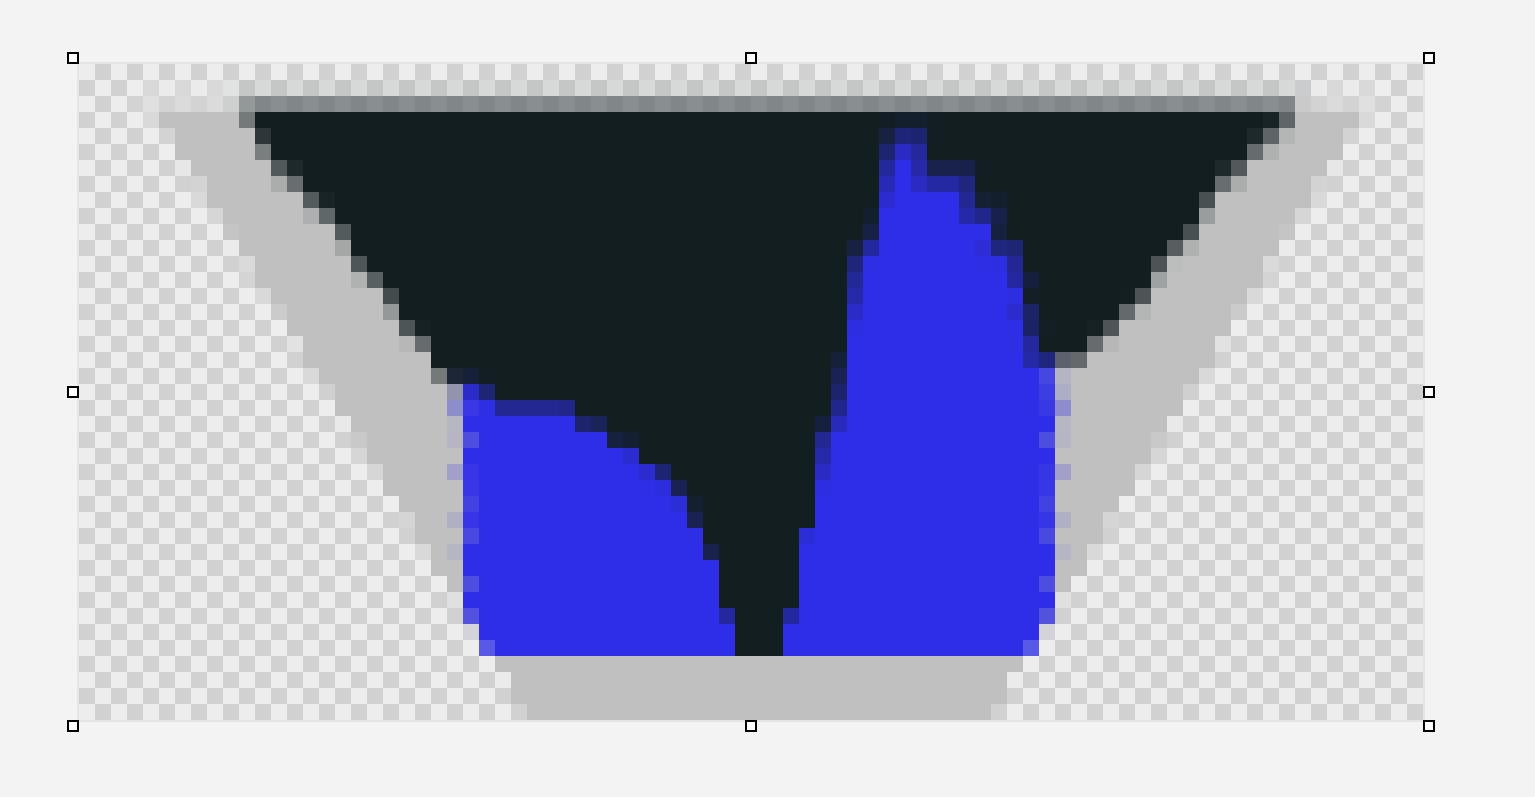
\includegraphics[width=50mm]{Photo/LiDAR/19.png}\\
    正面のタイルが正方形として映し出されるように修正した。
    \vskip.5\baselineskip
    \noindent
    さらにどこまでが壁(障害物)なのかを判断するためにLiDARのデータを画像上に適用する。\\
    このような処理を挟むのは、壁と床の境界を判別することでチェックポイントタイルなどの「灰色っぽい床」と「灰色っぽい障害物」を混同しないためである。\\
    下の画像のオレンジ色の点がLiADRの点である。\\
    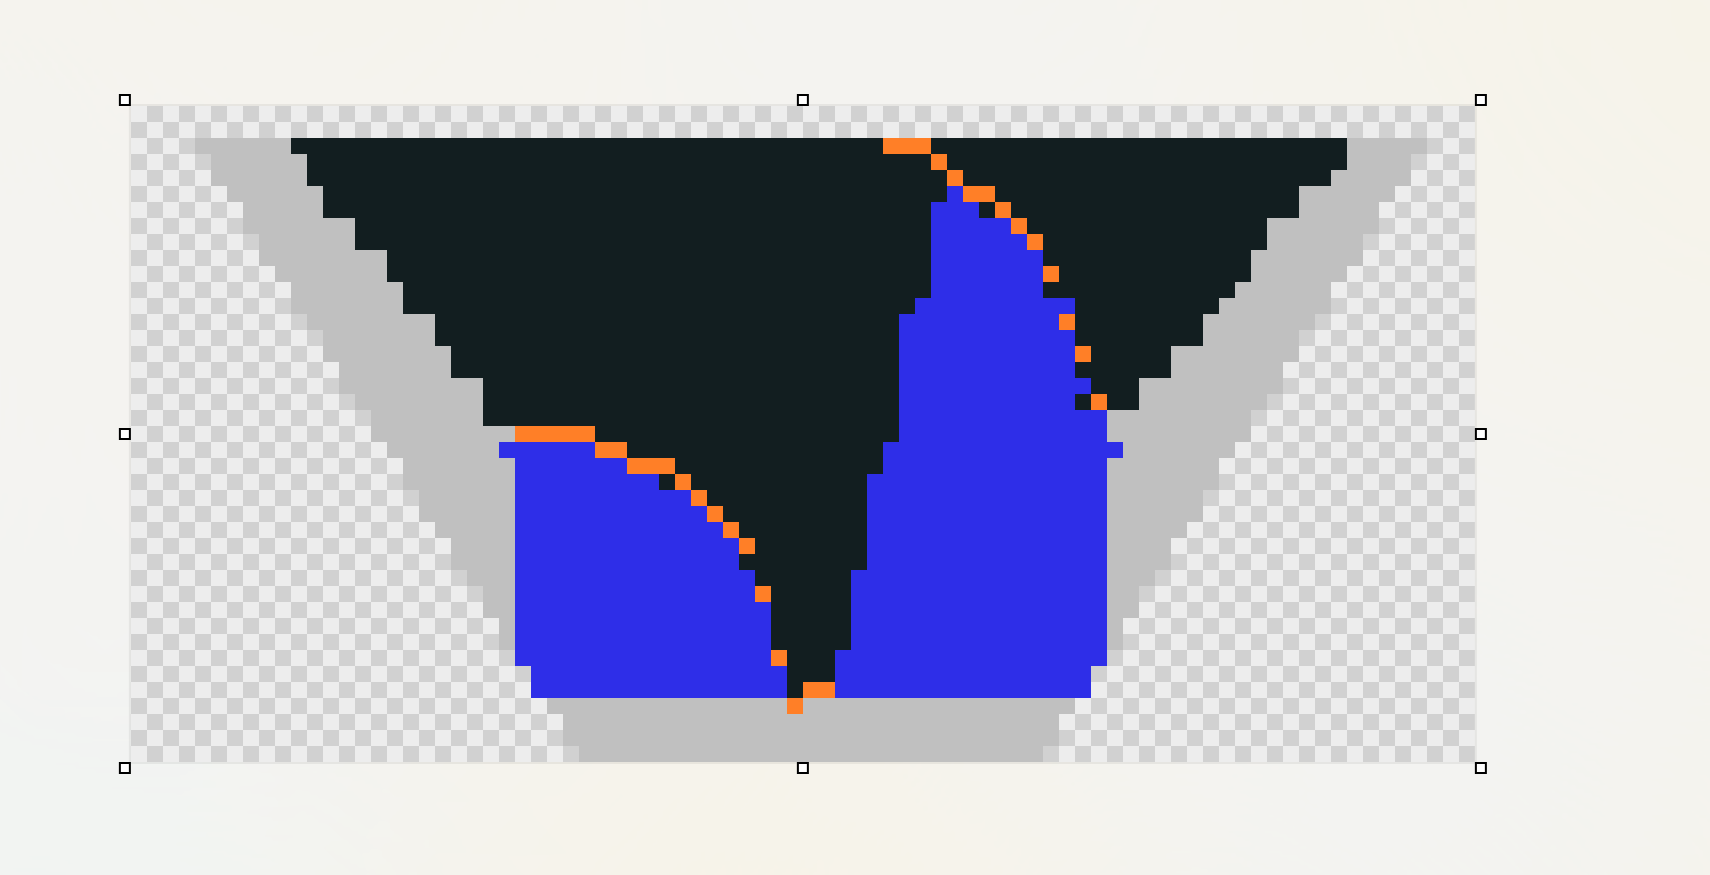
\includegraphics[width=50mm]{Photo/LiDAR/20.png}\\
    すると、この点よりも上にある部分は壁もしくは障害物であることが分かる。後は彩度が低ければ障害物、青よりの色であれば壁であると判断できる。
    \vskip.5\baselineskip
    \noindent
    障害物があった場合の例:\\
    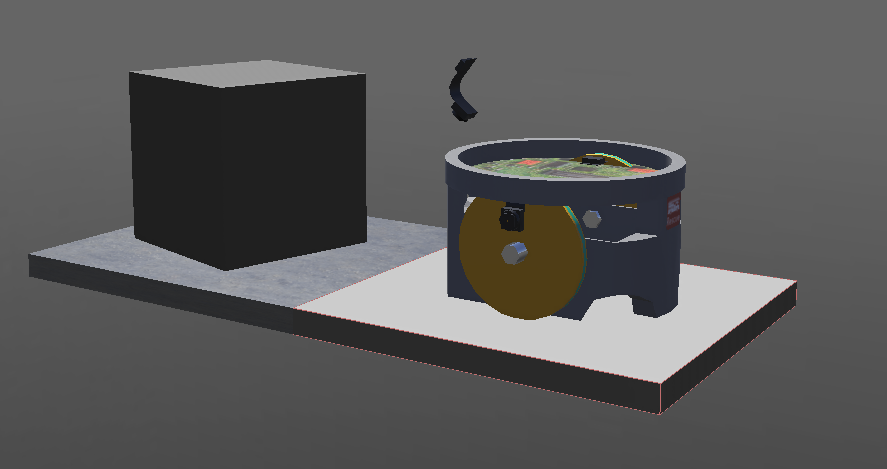
\includegraphics[width=40mm]{Photo/LiDAR/21.png}
    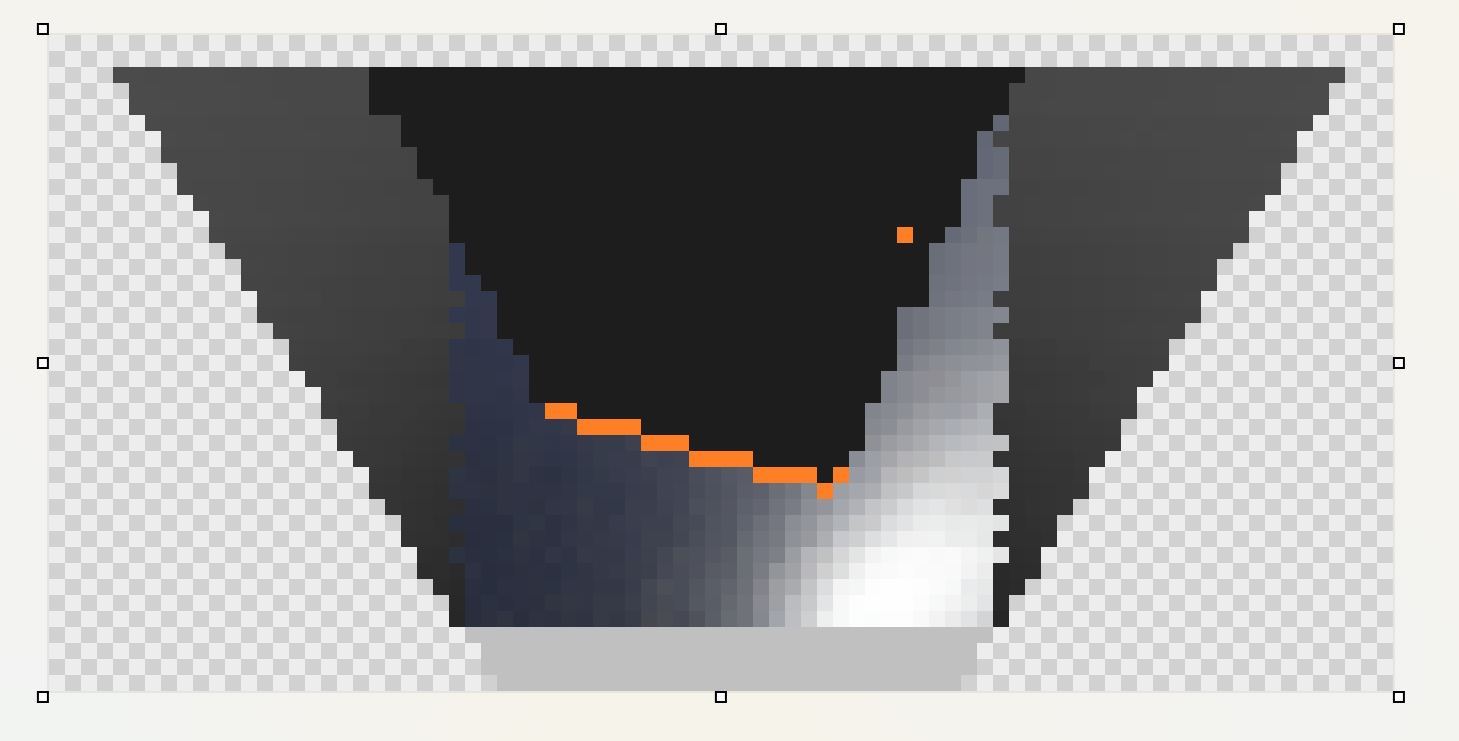
\includegraphics[width=40mm]{Photo/LiDAR/22.png}\\

    \subsection{床の色の識別}
    正面カメラの下側には自分のいるタイルが映っている。カメラを使うことで、機体が2枚のタイルを跨いでいるときでも左右それぞれの場合について判断することができる。\\
    また、カメラに手前のマスも写っていることで、落とし穴に差し掛かることなくこれを判断することができる。\\
    \vskip.5\baselineskip
    \noindent
    最も判断しづらいのは下のパターンだ。チェックポイントタイルの反射で床の色が一様でなく、さらに壁で見える床の面積も狭い。一番下でも17ピクセルしか判断材料がない。\\
    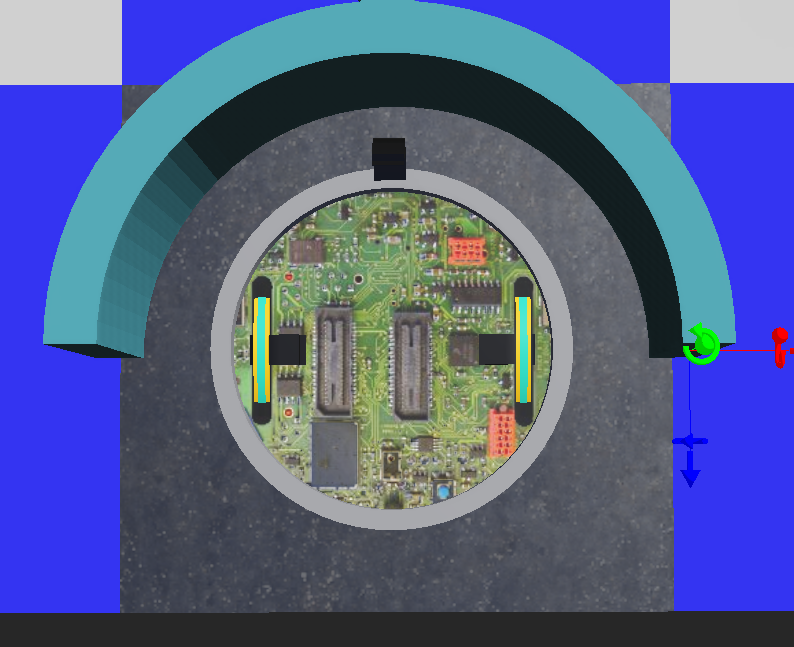
\includegraphics[width=40mm]{Photo/LiDAR/23.png}
    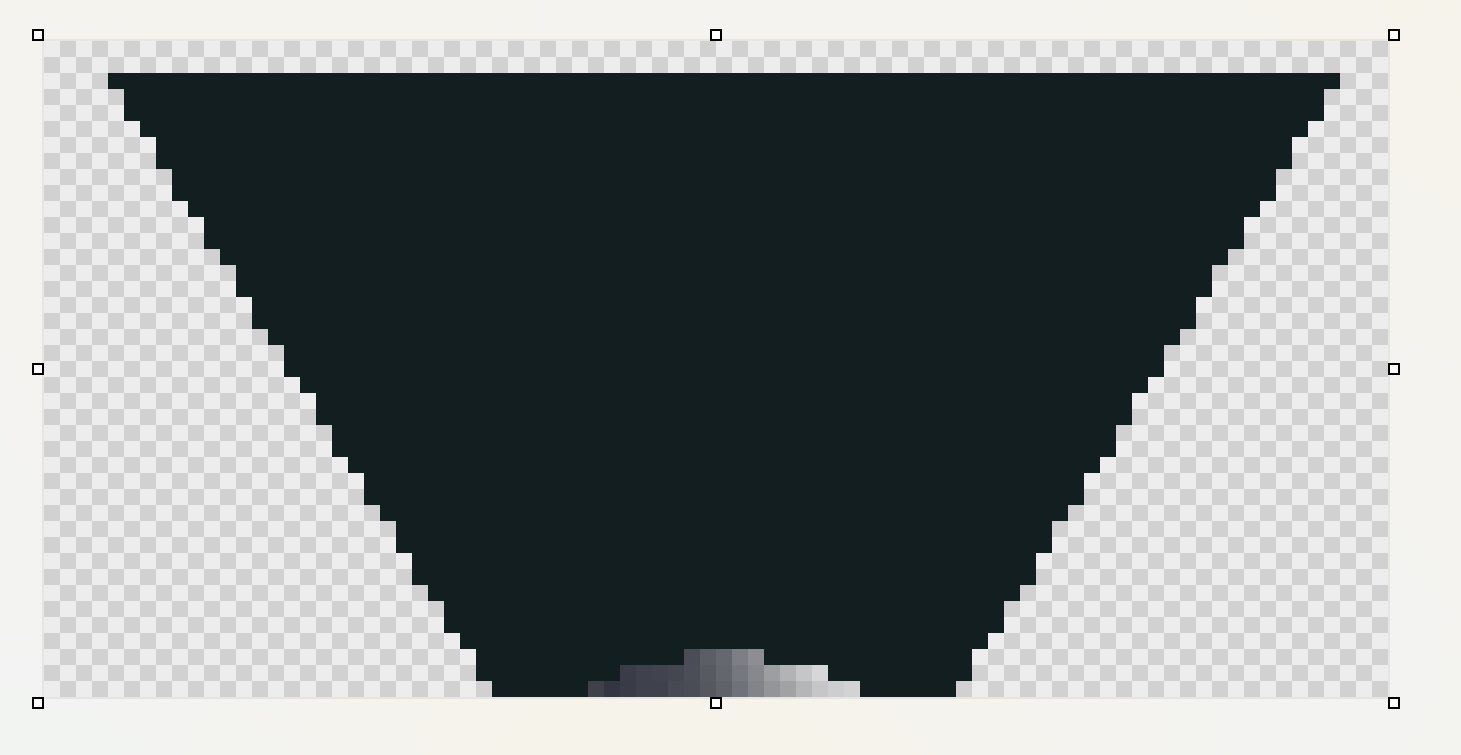
\includegraphics[width=40mm]{Photo/LiDAR/24.png}\\
    この場合、水色で示した範囲はタイルの境界の可能性があるため使えない。そこでオレンジ色で示したそれぞれ4ピクセルを用いる。\\
    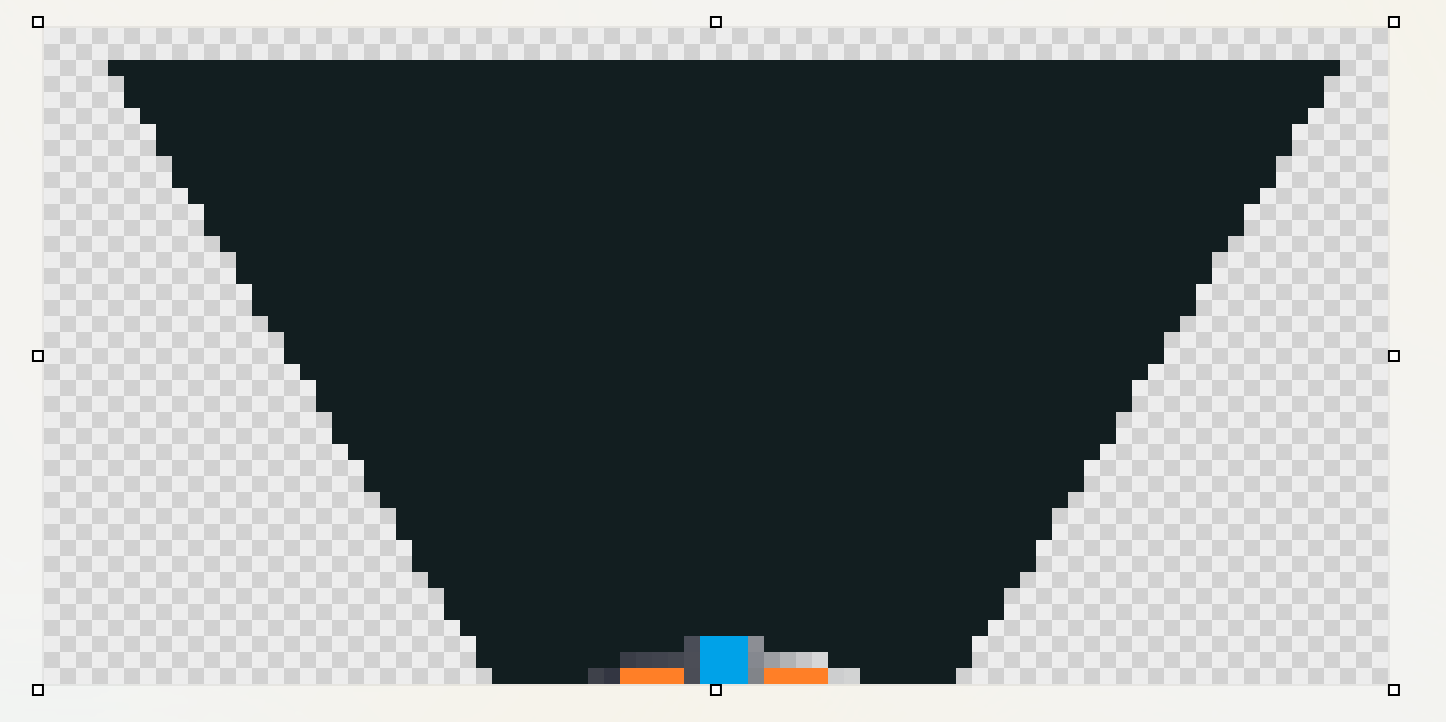
\includegraphics[width=40mm]{Photo/LiDAR/25.png}\\
    多くのタイルは画角のどこに映っても色が変化することはない。よってHSVを用いて狭い閾値でも判断できる。\\
    問題のチェックポイントタイルは彩度0かつ、明度の分散が大きいという条件で定義する。

    \subsection{落とし穴}
    「差し掛かる前に避ける」が基本方針である。\\
    LiDARによって進路を決定し、まずその進路を向く。この時障害物を検知を行い、それと同時に自分のいるタイルの色の判定、進む先のタイルの色の判定を行う。ここで壁の判定と一致しない障害物を発見した際には進路の修正を行う。\\
    進む先のタイルの色の判定については「落とし穴orそれ以外」のみのスケールで行う。\\
    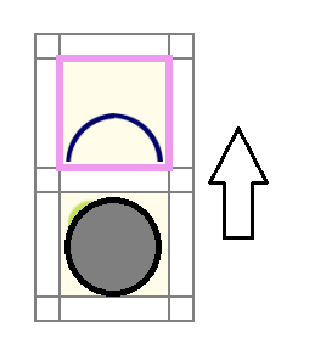
\includegraphics[width=30mm]{Photo/LiDAR/26.png}\\
    進行方向として選択された以上、最低でも上図のスペースは担保されているはずである。これを利用して自分のいるタイルの時よりも余裕をもって隣のタイルの色を判定することができる。\\
    左右について色の判定を行い、どちらか片方でも落とし穴と判定された場合はマップにそれを記録し、進路の訂正を行う。

  \section{被災者の発見}
    Pythonを手放したことによって便利なYoloやSSDなどの機械学習ライブラリが使えなくなってしまった。だが、一般的にはメイズ、シミュレーションを見渡しても機械学習が一般的なようだ。ここまでくると機械学習への反骨心が芽生えてきた。\\
    
    \subsection{事前処理}
    毎回毎回、被災者に関するすべての処理をしていると、制御周期が長くなりすぎてしまう。\\
    そこで、「どんな種類かわからないけど、何らかの被災者orハザードマップ」を判断してから、本格的な分類に入る。\\
    \vskip.5\baselineskip
    \noindent
    まず、前処理ではLiDARを使ってカメラの向いている方向に壁があるかを判断する。\\
    次に、エッジ検出をして直線に近似し、そこから四角形、ひし形を探す。\\
    これで四角形が見つかった場合はロボットの移動を停止して個別の判定に移る。
    \vskip.5\baselineskip
    \noindent
    ここで一時停止することによって、被災者救出の条件である1秒停止を始めることができる。その間に判別してしまえば処理にかかる時間は気にしなくてもよいということだ。
    
    \subsection{ハザードマップのF・O}
    これらは赤色、黄色と他にない色を持っている。\\
    そのため黄色があれば確実にO、赤が有って且つ黄色があれば確実にFであると判断できる。
    
    \subsection{その他の被災者、ハザードマップ}
    SIFTという方法を使って特徴点を抽出する。そしてその抽出した特徴点を、事前に撮影したものの特徴点とマッチングして、つながった特徴点の数が最も多いものを報告する。
    \vskip.5\baselineskip
    \noindent
    これは、まだまだ未完である。もし上手くいきそうになかったらOpenCVの機械学習→PyTorchの順で試すつもりだ。
  
  \section{工夫した点・苦労した点・アピールポイント}

    \subsection{読みやすいコードを}
    前回大会のコードの反省点、それは各マイコンのプログラムを1つのファイルに書いていたことだ。無造作に並ぶ千行近いコード。さよなら可読性。読みづらいったらありゃしない。\\
    この反省を基に、今回はファイルを複数に分割して作成した。\\
    具体的には、各センサ・モータのクラスをそれぞれ含んだファイル、マッピングのファイル、DFSのファイル...といった具合でモジュール単位に分けている。\\
    こうすることでカプセル化されたセンサやモータをDFSなどで簡単に使うことができ、可読性・保守性も向上する。\\
    また、書いたコードを「循環的複雑度」という指標を用いて定期的に評価した。

    \subsection{GPSトレース}
    ライントレースではラインを基準に走り、メイズでは距離センサを基準に走ることが多いだろう。だがこのプログラムではGPSを基準に走る。私はそれをGPSトレースと呼んでいる。\\
    関数の主な仕様は\\
    \begin{itemize}
      \item 目的地の座標と、速度を引数として関数に渡す
      \item 目的地の方向を自動で向く
      \item 目的地までの距離と経路からのズレを偏差としてPID制御
    \end{itemize}
    目的地と現在地の座標を比較し、Z軸方向との偏角が小さい場合は目的地のZ座標を経路として走り、X軸方向との偏角が小さい場合は目的地のX座標を経路として走る。
    \vskip.5\baselineskip
    \noindent
    斜め方向に目的地まで走るオプションもある。始点と目的地を結んだ直線をトレースするものである。経路からのズレ(偏差)を求めるには点と直線の距離公式から絶対値を除いた式を利用した。あえて絶対値を付けないことで現在地が直線の上下どちらにあるかを判別でき、そのままベクトル量の偏差として扱うことができる。
    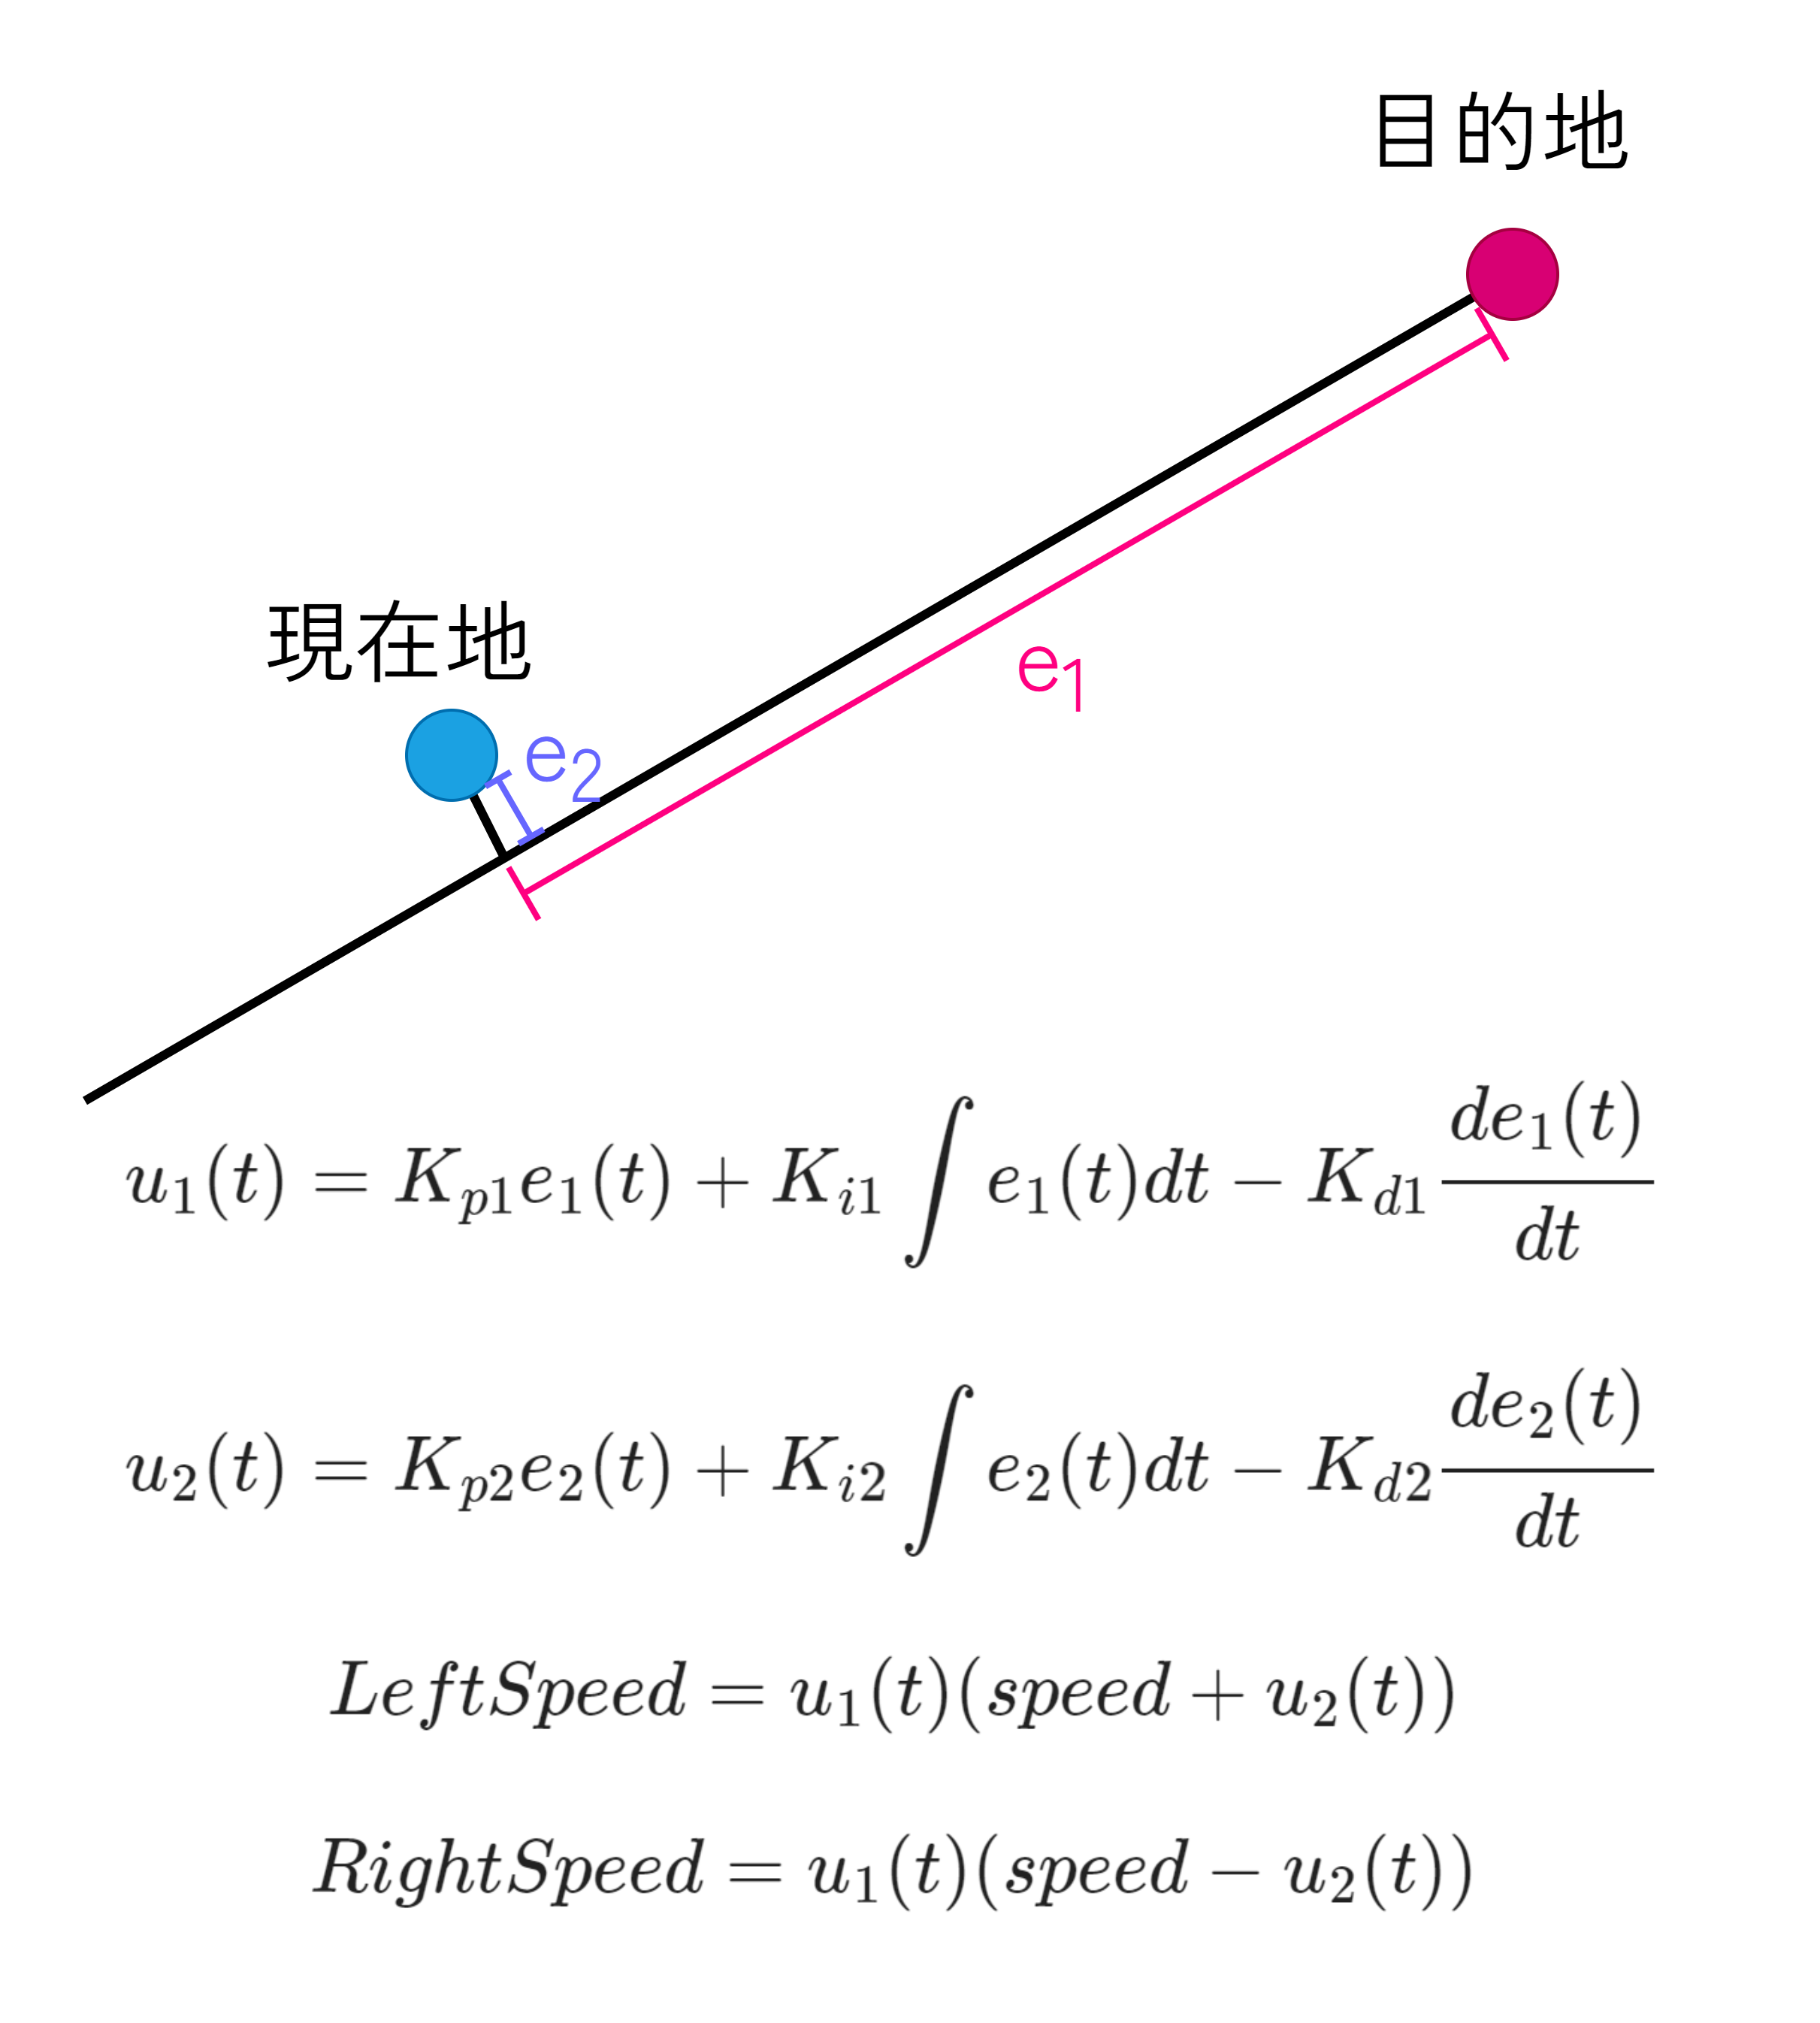
\includegraphics[width=50mm]{Photo/LiDAR/27.png}

    \subsection{壁マッチング}
    \noindent
    今回のプログラム内には採用されていないが、点群同士のマッチングをベースにした壁認識も開発した。
    \vskip.5\baselineskip
    \noindent
    ここでは約200パターンの壁を予め測定、モデルとしてプログラムに組み込む。この際、特徴量の1つとして中心から見た左右の点の数も記録する。\\
    この点の数は壁のパターンによって左右それぞれ5種類ほどに分類でき、これを基にフィルターをかけることでマッチングの対象となるモデルを元の約200個から10個程度に抑えることができる。\\
    マッチングは中央から見た左右に分けて行う。左右それぞれでマッチングする点を3回ずらしながら累積2乗誤差を記録し、それが最も小さいものをそのモデルの「偏差」として記録する。そしてその偏差が最も小さかったモデルを採用する。
    \vskip.5\baselineskip
    \noindent
    この手法の問題点として以下のものが挙げられた。
    \begin{enumerate}
      \item 機体の位置ずれによって点の数が増減した場合に対処できない。
      \item 向きによって壁の生成パターンが違う。
      \item タイルの中心でない(1/2タイル進んだ状態)でも生成規則が違う。
      \item 測定誤差による累積2乗偏差が壁の違いによるそれを上回る。
    \end{enumerate}
    1.はICPなどで使用される最近傍探索の技術で解決できる。2.3.はそのパターンをコードに組み込んでしまえば解決できる上に、その微妙な違いによって本来見えない裏側の壁まで判定できる。\\
    しかし、4.を解決できなかったため今回の採用は断念した。SLAMなどで使用される点群と点群同士のマッチングは測定対象が一部一致する2つの比較であったのに対して、今回は多数の不正解から正解を探す比較である。前提条件が違ったのだ。
    \vskip.5\baselineskip
    \noindent
    ちなみにモデルはこのように保存されている。\\
    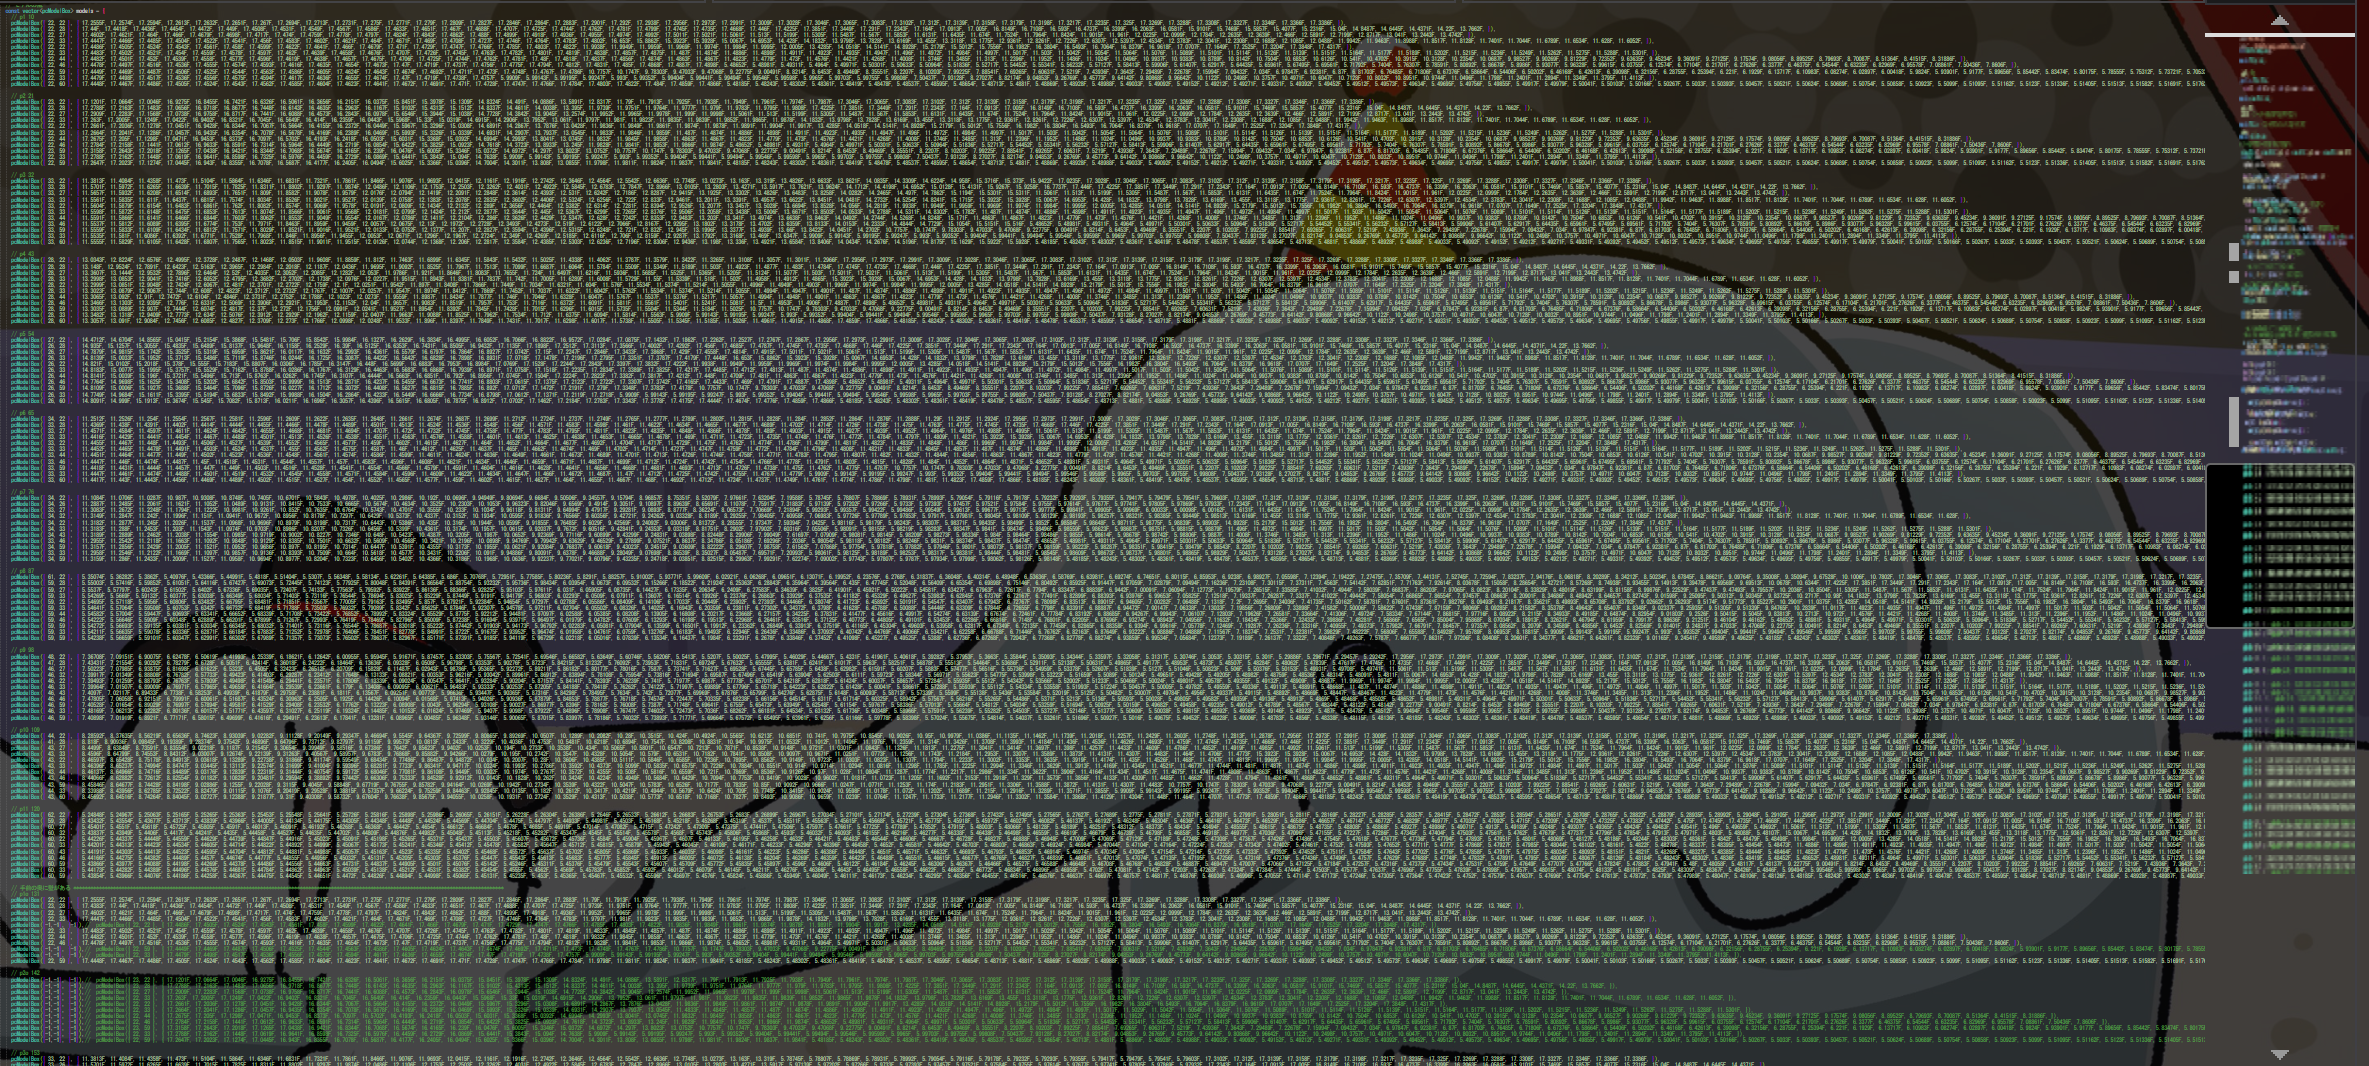
\includegraphics[width=150mm]{Photo/LiDAR/28.png}

    \subsection{空間把握}
    \noindent
    これも現時点でプログラム内には採用されていないものである。
    フィールド内で広い空間(2*3とか)に出くわした時、それを普通に回るのでは効率が悪いと考え、その空間サイズを把握できるような関数を書いた。\\
    これまでの関数は「点」を基準に書いてきたが、それでは下の画像の青い線で示されたところを判断できない。\\
    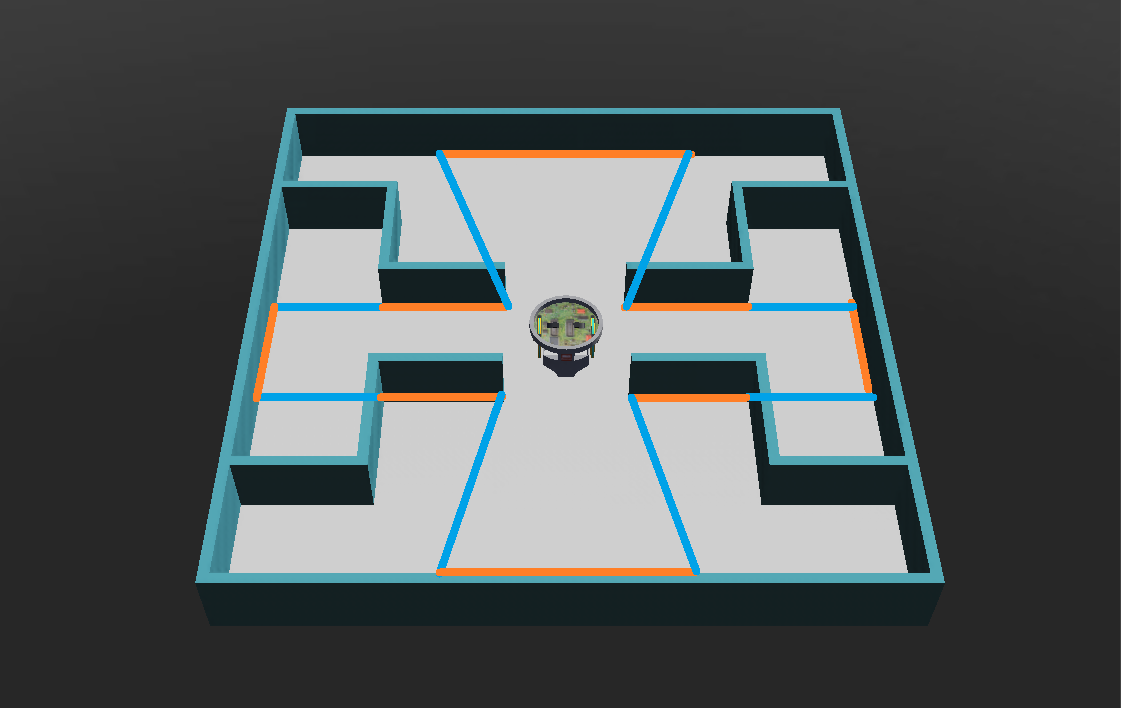
\includegraphics[width=100mm]{Photo/LiDAR/29.png}\\
    そこで「線」を基準に考える。ある意味正しい空間把握はできないが、最低限自分の周りの空間サイズまでは把握できる。\\
    判定方法は「壁認識」の「9. 斜めに進むという選択肢」でも説明した直径7cmの円を線にぶつかるかで動かすという方法。そして指定した範囲の線を切り取ってそこから距離を判断する方法がある。
    \vskip.5\baselineskip
    \noindent
    ただ、そのサイズはロボットが動くラビに時々刻々と変化してしまう。それ対応するのが難しく使用できていない。

    \subsection{数学的視点}
    今年の大会において痛感したのが、数学の偉大さだ。分散・微分・三角関数などを使うという発想は高校数学をちゃんと履修した賜物だと考えている。\\
    普通に生きている分にはその存在を感じさせない彼だが、現代社会を根底で支えていることを深く感じさせられた。\\
    今後も数学を学び続けるモチベーションになったように思う。

\end{document}